%\documentclass[12pt,a4paper,twoside]{book}
\documentclass[12pt,a4paper]{book}

% includes
\usepackage[inner=2cm,outer=2cm,top=3cm,bottom=3cm]{geometry}
%\usepackage[inner=3cm,outer=3cm,twoside,top=3cm,bottom=3cm]{geometry}
%\usepackage[inner=2cm,outer=3cm,twoside,top=3cm,bottom=3cm]{geometry}
\usepackage[utf8]{inputenc}
\usepackage[english]{babel}
\usepackage{mathtools}
\usepackage{amssymb}
\usepackage{amsthm}
\usepackage{amsmath}
\usepackage[unicode]{hyperref}
\usepackage{indentfirst}
\usepackage{aliascnt}
\usepackage{chngcntr}
\usepackage{stmaryrd}
%\usepackage{graphicx}
\usepackage{subcaption}

\usepackage{tikz}
\usetikzlibrary{positioning,arrows}
\usepackage[citestyle=alphabetic,style=numeric]{biblatex}
%\usepackage[nottoc]{tocbibind} for bibliography in the toc (??? TODO)
%\usepackage{booktabs}   for better tables (TODO)
%\usepackage{pdfpages} to include external pdf in the latex document
%\usepackage{stackengine}
%\stackMath

\usepackage{enumitem}

% TODO check all
%\RequirePackage{faktor} for better fractions (eg num and denom doesn't get smaller)
%\RequirePackage{wasysym} a font
%\RequirePackage{fancyhdr} for things with header
%\RequirePackage{lipsum} to get lorem ipsum
%\RequirePackage{titlesec}for thing on section headers and titles
%\RequirePackage{setspace} for spacing between lines (it works also without?)
%\RequirePackage{mdframed} thinghs for framed, maybe needed by tikz
%\RequirePackage{minted}
%\RequirePackage{url}
%\RequirePackage{xcolor} better color handling, maybe needed by code ?

\usepackage{todonotes}
% Epigraphs
%\makeatletter
%\newenvironment{epigraph}[2][2em]
%{\setlength{\@tempdima}{#1}%
%	\def\chapquote@author{#2}%
%	\parshape 1 \@tempdima \dimexpr\textwidth-2\@tempdima\relax%
%	\itshape}
%{\par\normalfont\hfill--\ \chapquote@author\hspace*{\@tempdima}\par\bigskip}
%\makeatother
% ======================== Package for syntax highlight ===========================
\usepackage{csquotes}
\usepackage{minted}

\graphicspath{{images/}}
\setlength{\parindent}{0.5cm}     % paragraph indentation
\linespread{1.2}                % space between lines

\addbibresource{bibliography/tot.bib}

\hypersetup{linktocpage}

% COMMANDS
\definecolor{light-gray}{gray}{0.95}
\newcommand{\code}[1]{\colorbox{light-gray}{\texttt{#1}}}
\newcommand{\labelitem}[1]{\item[] \textit{#1}:}
\newcommand{\setN}{\mathbb{N}}
\newcommand{\setZ}{\mathbb{Z}}
\newcommand{\svert}{\,\vert\,}
\newcommand{\pow}{\mathcal{P}}
\newcommand{\fix}{\text{fix}}
\newcommand{\id}{\text{id}}
\newcommand{\lfp}{\text{lfp}}
\newcommand{\op}{\text{op}}
\newcommand{\image}{\text{Im}}
\newcommand{\Int}{\text{Int}}
\newcommand{\poly}{\text{poly}}
\newcommand{\drop}{\text{drop}}
\newcommand{\concat}{\text{concat}}

\newcommand{\macheps}{\textbf{u}}
\newcommand{\fp}{\text{fp}}

\DeclarePairedDelimiter{\denot}{\llbracket}{\rrbracket}
\DeclarePairedDelimiter{\abs}{\lvert}{\rvert}

% Theorems
\theoremstyle{plain}
\newtheorem{theorem}{Theorem}
\counterwithin{theorem}{chapter}

\newtheorem{corollary}[theorem]{Corollary}
\providecommand*{\corollaryautorefname}{Corollary}

\newtheorem{lemma}[theorem]{Lemma}
\providecommand*{\lemmaautorefname}{Lemma}

\newtheorem{prop}[theorem]{Proposition}
\providecommand*{\propautorefname}{Proposition}

\theoremstyle{remark}
\newtheorem{remark}[theorem]{Remark}
\providecommand*{\remarkautorefname}{Remark}

\newtheorem{example}[theorem]{Example}
\providecommand*{\exampleautorefname}{Example}

\theoremstyle{definition}
\newtheorem{definition}[theorem]{Definition}
\providecommand*{\definitionautorefname}{Definition}

\begin{document}
	% macros (global)
	\newcommand{\speciality}    {Informatica}
\newcommand{\promotion}     {2021}                                  %<---------

\newcommand{\thesistitle}   {TBD}    %<---------

\newcommand{\authorlast}    {Ascari}                               %<---------
\newcommand{\authorfirst}   {Flavio}
\newcommand{\authornamefl}  {\authorfirst \space \authorlast} % first name first
\newcommand{\authornamelf}  {\authorlast \space \authorfirst} % last name first
\newcommand{\authorbirth}   {08 dicembre 1997}                      %<---------
%\newcommand{\authoraddress} {---} %<---------
%\newcommand{\authorcnp}     {1234567891234}                         %<---------

\newcommand{\peopleheader}  {Candidate \hfill Supervisors \\}
\newcommand{\supervisors}   {Roberto Bruni \\ \hfill Roberta Gori}               %<---------

	% front-matter
	\pagenumbering{gobble}

	% define the cover page
\begin{titlepage}
	\begin{center}
		
\includegraphics[width=0.45\textwidth]{marchio_unipi.eps}

		\vspace{1cm}
		\large
		\textbf{\MakeUppercase{Department of Computer Science}}\\
		\textbf{Master Degree in Computer Science}

        % thesis title
		\vspace{3cm}
		\Large
		\textbf{\MakeUppercase{Thesis}}

		\vspace{0.5cm}
		\LARGE
		\textbf{\thesistitle}

		% author and relator
		\vspace{3.5cm}
		\Large
		\peopleheader
		\textbf{\authornamefl} \hfill \textbf{\supervisors}        

		% session
		\vfill
		\large
		\textbf{\MakeUppercase{Academic year 2020/2021}}
    \end{center}
\end{titlepage}
	\cleardoublepage

	\thispagestyle{plain}
\begin{center}
	\Large
	\textbf{\thesistitle}

%	\vspace{0.4cm}
%	\large
%	Thesis Subtitle

	\vspace{1.2cm}
	\large
	\peopleheader
	\textbf{\authornamefl} \hfill \textbf{\supervisors}

	\vspace{2.0cm}
	\textbf{Abstract}
\end{center}
Static program analyses are a set of useful techniques that allows to infer properties on programs from their source code, without executing them. Among those, abstract interpretation is a general framework to define sound analyses based on constructive approximations that found its way through many aspects of modern Computer Science.
Nowadays most formal static analyses focus on over-approximation, that is they determine a set bigger than the set of all possible behaviours of the program, in order to show absence of bugs: if the analysis reports no unwanted behaviour, then the program doesn't have any.
In principle there is another, dual application of static analyses: to compute and under-approximation of the set of possible behaviours in order to find bugs. However, this kind of analyses hasn't been studied as intensively as over-approximations in the last few decades, and even though abstract interpretation has been proposed for over as well as under-approximation, in practice has almost only been used for the former.

In this thesis, we would like to investigate both technical and conceptual reasons that make the design of under-approximation abstract domains difficult. We present the main differences between over and under-approximation, and we propose the new definition of ``non emptying function" to describe a function whose analysis produces a non vacuous result. Using this definition, we give conditions for the non existence of under-approximation domains. Lastly, we study the limitations of approaches that use this definition in order to prove non existence of such domains.


	% table of contents
	\tableofcontents

	% chapters
	\setcounter{page}{1}
	\pagenumbering{arabic}

	\chapter{Introduction}

Thesis introduction.

\section{Abstract interpretation}
Static program analyses are a useful set of techniques to infer properties of programs from their source code, without executing them. Among those, abstract interpretation (\cite{cousot-77}\cite{cousot-79}) is a general framework to design analyses sound-by-construction.

Introduced for both over- and under-approximations, but used only for the former.\cite{cousot-77}\cite{cousot-79}

\begin{example}[Intervals]\label{intr:ex:intervals}
	\todo{Intuitive description of interval based analysis}
\end{example}

\section{Under-approximations}
Recent interest in under-approximations (see eg. \cite{ohearn-incorrectness-logic}), we would like to investigate whether this can be done in the setting of abstract interpretation.

\section{Contributions}
Brief description of the thesis subjects, highlighting new contributions/approaches. Chapters overview.

The goal of this thesis is to investigate the reasons that prevented the development of an under-approximation theory within the abstract interpretation framework.

We think one of the reasons this haven't happened is that "recover" from bottom is way harder than from top.
	\chapter{Background}

Things needed to understand the thesis that aren't strictly related to the thesis subject.

\section{Notation}
\todo{probably drop this section}
$C (\alpha, \gamma) A$ means a Galois Connection (GC) between $C$ and $A$.

If $S$ is a poset, $S^{\op}$ is the poset with the opposite ordering. So for instance $\pow(C)^{\op}$ is the powerset of $C$ ordered by containment $\supseteq$, and hence $\emptyset$ is the greatest element ($\top$) of the set.

Unless otherwise specified, a Galois Insertion (GI) is always specified with the ``small" set on the right, ie. if $C (\alpha, \gamma) A$ is a GI then $\alpha \circ \gamma = \id_A$.

Given a GC $C (\alpha, \gamma) A$, an element $c \in C$ is \textit{representable} in $A$ if $\gamma(\alpha(c)) = c$.

%Given $\pZop (\gamma, \alpha) A$ a GI, we call $n^{\flat}$ the only abstract element (if any) such that $\gamma(n^{\flat}) = \{ n \}$. We say $n^{\flat} \notin A$ if there is no such element in $A$.

Recall that in a GI $\gamma$ and $\alpha$ map concrete top in abstract top and vice versa.

A GI is the same as assuming $A \subseteq C$, and we'll do this. With this notation, $f^{\#}$ is the same as $\alpha \circ f$, but is conceptually different.

Given a function $f : C \rightarrow D$ we use the same symbol also to denote its additive extension $f: \pow(C) \rightarrow \pow(D)$.

Meaning of $\infexists$.

\section{Partially ordered sets}
This section recalls basic notions of order theory upon which (much of) the abstract interpretation framework is based. For a more comprehensive introduction to order theory, we refer the reader to a text book, such as for instance \cite{order-theory-book} or appendix A of \cite{principles-of-program-analysis-book}.

\begin{definition}[Partial order]
	Given a set $S$, a partial order $\preceq$ on $S$ is a relation on it that, for all $a$, $b$ and $c$ in $S$, satisfies
	\begin{itemize}
		\labelitem{reflexivity} $a \preceq a$
		\labelitem{antisymmetry} if both $a \preceq b$ and $b \preceq a$ then $a = b$
		\labelitem{transitivity} if both $a \preceq b$ and $b \preceq c$ then also $a \preceq c$
	\end{itemize}
\end{definition}
We say that the pair $(S, \preceq)$ is a partially ordered set, or a \textit{poset} for short, and we usually write only the carrier set $S$ when the ordering is unambiguous.

\begin{definition}[Opposite ordering]
	Given a poset $(S, \preceq)$, the \textit{opposite} poset $(S, \preceq^{-1})$ is defined with $a \preceq^{-1} b$ if and only if $b \preceq a$.
\end{definition}
We often use $\succeq$ to indicate $\preceq^{-1}$ and $S^{\op}$ for (the carrier set of) the opposite poset.

\begin{definition}[Upper bounds and least upper bound]
	Given a poset $S$ and one of its subsets $T \subseteq S$, an \textit{upper bound} of $T$ is an element $c \in S$ that is greater or equal than any element of $T$:
	\[
	\forall a \in T.\ a \preceq c
	\]
	The \textit{least upper bound} (or lub for short) of $T$, if it exists, is an upper bound of $T$ that is smaller or equal than all other upper bounds of $T$.
\end{definition}
In general a set $T$ needs not have a least upper bound, but when it does it's unique and we denote it with $\bigsqcup T$. Moreover, when $T = \{ a, b \}$ is made of just two elements, we shall write $a \sqcup b$ for their least upper bound.

The dual notion of lub is that of glb:
\begin{definition}[Lower bounds and greatest lower bound]
	Given a poset $S$ and one of its subsets $T \subseteq S$, a \textit{lower bound} of $T$ is an element $c \in S$ that is smaller or equal than any element of $T$:
	\[
	\forall a \in T.\ c \preceq a
	\]
	The \textit{greatest lower bound} (or glb for short) of $T$, if it exists, is a lower bound of $T$ that is greater or equal than all other upper bounds of $T$.
\end{definition}
Again, if this exists we denote it with $\bigsqcap T$, and if $T = \{ a, b \}$ we use the notation $a \sqcap b$.

\begin{definition}[Lattice]
	A poset $S$ is called a \textit{lattice} if every pair of elements has a lub and glb. It is called a \textit{complete lattice} if every subset has a lub and a glb.
\end{definition}

\begin{definition}[Monotone function]
	Given two poset $S$, $T$ and a function $f : S \rightarrow T$, that function is called \textit{monotone} (or \textit{order-preserving}) if, for any pair $a, b \in S$ of elements of the domain such that $a \preceq_S b$, also their images satisfies $f(a) \preceq_T f(b)$.
\end{definition}

Given a set $S$ and a poset $T$, we can consider the set of functions from $S$ to $T$. This has a natural structure of poset too.
\begin{definition}
	Given two functions $f, g: S \rightarrow T$, we say that $f \preceq g$ if for all elements $a \in S$ we have
	\[
	f(a) \preceq g(a)
	\]
\end{definition}
It's easy to show that this relation among functions is a partial order too. Moreover, if $T$ is a (complete) lattice, the set of functions from $S$ to $T$ is a (complete) lattice too, and this still holds if $S$ is a poset and we restrict ourselves to monotone functions between the two.

\section{Galois connections}
\todo{add references for this whole section}
The main mathematical tool we use to study abstract interpretations are Galois connections, and the special case of Galois insertions.

\begin{definition}[Galois connection]\label{ch2:def:gc}
	Let $C$ and $A$ be two partially ordered sets, and $\alpha : C \rightarrow A$, $\gamma : A \rightarrow C$ be a pair of monotone functions between the two.
	
	We say $C (\alpha, \gamma) A$ is a Galois connection if, for any choice of $c \in C$ and $a \in A$ we have
	\[
	\alpha(c) \preceq a \iff c \preceq \gamma(a)
	\]
\end{definition}

For our goals, we will call $C$ the \textit{concrete domain}, $A$ the \textit{abstract domain}, $\alpha$ the \textit{abstraction function} and $\gamma$ the \textit{concretization function}. The two functions $\alpha$ and $\gamma$ are also called \textit{adjoints}\footnote{Actually the term ``adjoint" comes from Category Theory, since Galois connections are adjunctions between the two posets seen as categories. However such a discussion would be outside the scope of this thesis, and would also require a basic knowledge of category theory.}.

\todo{Add meaning of the order on $C$ and $A$}
In program analysis we give the following intuitive meaning to those. $C$ is the domain of concrete states, $A$ the set of abstract properties we're interested in, $\alpha$ the function that maps a concrete state in the most precise abstract property that describes it and $\gamma$ a function that maps an abstract property in the biggest concrete state it describes.

\begin{example}[Intervals]\label{ch2:ex:intervals}
	We can now formalize the intuitive example \ref{intr:ex:intervals} of intervals we introduced in the previous chapter.
	$C$ is the set of possible values of the variable \code{x}. Since this is an integer values, elements of $C$ are subsets of $\setZ$, so $C = \pow(\setZ)$, with the ordering given by set inclusion. $A$ is the set of abstract properties we track in our analysis, so in our example the set of interval to which \code{x} may belongs. This means $A = \Int$.
	$\alpha$ is the function that allows us to abstract a set of possible values of \code{x} into the best (ie. most precise) possible abstract property:
	\begin{align*}
		\alpha(S) &= [\min(S); \max(S)]
	\end{align*}
	with the convention that $\min(\emptyset) = +\infty$, $\min(\emptyset) = -\infty$, the minimum of a lower-unbound set is $-\infty$ and the maximum of an upper-unbound set is $+\infty$. This abstraction function is exactly what we expect: no smaller interval can describe the set $S$, since $\min(S)$ and $\max(S)$ are elements of $S$ and so must also be in the interval. Conversely, this is a correct abstraction of $S$ since all its elements are between $\min(S)$ and $\max(S)$, so are in the interval too.
	
	$\gamma$ is the function that does the inverse operation: given an interval $[n, m]$, thought as a formal writing that describes the property that the value of \code{x} is between $n$ and $m$, gives us its ``meaning", that is the largest subset of $\setZ$ that matches that property:
	\[
	\gamma([n, m]) = \{ x \in \setZ \svert n \le x \le m \}
	\]
	The set $\{ x \in \setZ \svert n \le x \le m \}$ is exactly what is commonly represented with $[n; m]$: $\gamma$ is simply translating the formal writing (or, in our context, an abstract property) to a semantic set of values.

	Of course this definition of $\gamma$ is incomplete, the full, formal one being
	\begin{align*}
		\gamma([n, m]) &= \{ x \in \setZ \svert n \le x \le m \} \\
		\gamma([-\infty, m]) &= \{ x \in \setZ \svert x \le m \} \\
		\gamma([n, +\infty]) &= \{ x \in \setZ \svert n \le x \} \\
		\gamma([-\infty, +\infty]) &= \setZ \\
		\gamma([+\infty, -\infty]) &= \emptyset
	\end{align*}

	Showing that $\pow(\setZ) (\alpha, \gamma) \Int$ is a Galois connection is just a straightforward check. Fixed $S \in \pow(\setZ)$ and the interval $[n, m] \in \Int$ (for simplicity, we assume both $n$ and $m$ finite) we have
	\begin{align*}
		& \alpha(S) \preceq [n, m] \\
		\iff &[\min(S); \max(S)] \preceq [n, m] \\
		\iff &n \le \min(S),\, \max(S) \le m \\
		\iff &\forall x \in S\ .\ n \le x,\, \forall x \in S\ .\ x \le m \\
		\iff &S \subseteq \{ x \in \setZ \svert n \le x \le m \} \\
		\iff &S \subseteq \gamma([n, m])
	\end{align*}
\end{example}

We recall here two properties of Galois connection that will be useful in this thesis.

\begin{prop}\label{ch2:th:gc-extensive-charact}
	Let $C$ and $A$ be two partially ordered sets, and $\alpha : C \rightarrow A$, $\gamma : A \rightarrow C$ be a pair of monotone functions between the two.
	
	Then $C (\alpha, \gamma) A$ is a Galois connection if and only if both $\id_C \preceq \gamma \circ \alpha$ and $\alpha \circ \gamma \preceq \id_A$.
\end{prop}
\begin{prop}\label{ch2:th:gc-adjoints-preserve-glb-lub}
	Let $C (\alpha, \gamma) A$ be a Galois connection. Then $\gamma$ preserves greatest lower bounds and $\alpha$ preserves least upper bounds.
\end{prop}
In particular, this means that $\gamma$ maps $\top_A$ in $\top_C$ (because they are glb of the empty set) and dually $\alpha$ maps $\bot_C$ in $\bot_A$.

In a Galois connection it may very well happen that two abstract elements have the same concretization, as shown in the following example:
\begin{example}[Product abstraction]
	Consider two concrete domains, for instance two copies of $\pow(\setZ)$ that describes the possible states of two different variables \code{x} and \code{y} that appear in the program.
	Then consider the Galois connection $\pow(\setZ) (\alpha, \gamma) \Int$, and suppose we want to use it to abstract both variables. If we abstract separately both the element of $\pow(\setZ_x)$ and that of $\pow(\setZ_y)$ (where subscripts indicates the variable the domain refers to), we get a pair of intervals, one for \code{x} and one for \code{y}, that is an element of $\Int_x \times \Int_y$. It's easy to check that this abstraction function defines a Galois connection between $\pow(\setZ_x \times \setZ_y)$ and $\Int_x \times \Int_y$.
	
	However, this abstraction has redundant elements: consider
	\begin{align*}
		(\bot, [n, m])
	\end{align*}
	\[ ([n, m], \bot) \]
	\[ (\bot, \bot) \]
	where $\bot = [+\infty, -\infty]$ describes the empty interval. All these elements are concretized in the concrete $\emptyset \in \pow(\setZ_x \times \setZ_y)$.
\end{example}

We would like not to have those since they are different elements of the abstract domain that describes the same property. In analogy with logic, this is the same kind of redundancy as the possibility to describe the empty set in the following three different ways:
\[
\{ (x, y) \svert x \in \emptyset, n \le y \le m \}
\]
\[
\{ (x, y) \svert n \le x \le m, y \in \emptyset \}
\]
\[
\{ (x, y) \svert x \in \emptyset, y \in \emptyset \}
\]

In order to avoid this issue, we require $\gamma$ to be injective, so that no two different abstract elements can be concretized into the same concrete element, ie. they describe the same property. This turns out to give rise to an interesting definition, that of Galois insertion.
\begin{definition}[Galois insertion]\label{ch2:def:gi}
	Let $C (\alpha, \gamma) A$ be a Galois connection. We say this is a \textit{Galois insertion} if $\gamma$ is injective.
\end{definition}

The one proposed above isn't the standard definition of Galois insertion: more commonly, it requires $\alpha \circ \gamma$ to be identity on the abstract domain $\id_A$. However, the two are equivalent, as shown by the following characterization of Galois insertions.
\begin{prop}\label{ch2:th:gi-charact}
	Let $C (\alpha, \gamma) A$ be a Galois connection. Then the following are equivalent:
	\begin{enumerate}[label={(\arabic*)}]
		\item $\alpha \circ \gamma = \id_A$
		\item $\alpha$ is surjective
		\item $\gamma$ is injective
	\end{enumerate}
\end{prop}

The interval domain presented above is an example of Galois insertion: since we required $n \le m$ in the interval $[n, m]$ no two intervals describe the same concrete set, and hence $\gamma$ is injective. However, as we've seen, composing two independent interval domains gives rise to a Galois connection that isn't an insertion. There are techniques to delete redundant elements of an abstract domain in order to make it a Galois insertion (\todo{add references}), but we're not interested in them for this thesis.

In a Galois insertion, since $\gamma$ is injective, we have a bijection between $A$ and $\gamma(A)$. By the definition of Galois insertion we have $\alpha \circ \gamma = \id_A$, hence $\alpha$ is the inverse of $\gamma$ when restricted to $\gamma(A)$. Since both functions are monotone this defines an isomorphism of poset between $A$ and $\gamma(A) \subseteq C$.

Using this isomorphism, whenever we consider a Galois insertion we identify $A$ and its image, so that $A$ becomes a subset of $C$ and $\gamma = \id_A$. In this case, by proposition \ref{ch2:th:gc-extensive-charact} we have $\id_C \preceq \gamma \circ \alpha = \alpha$, corresponding to the intuitive idea that $\alpha$ must abstract a set of states in something bigger in order to over-approximate it.

Do note that this identification simplifies notation, but introduces a pitfall: reasoning as above we may be tempted to say that also $\alpha = \alpha \circ \gamma \preceq \id_A$, always by proposition \ref{ch2:th:gc-extensive-charact}, so concluding that $\id \preceq \alpha \preceq \id$ and hence $\alpha = \id$. However here we're neglecting the fact that $\gamma = \id_A$, not the identity on the whole set $C$, and actually $\gamma$ is defined only on elements of $A \subseteq C$. This means that the above relation is indeed correct, but only for elements of $A$, as pointed out by the fact that $\alpha \preceq \id_A$ and not $\id_C$. This is a problem that arise in general with this notation: two functions that looks the same are actually different because of their domain, that isn't specified. We'll make sure to always clarify the domain whenever it's not uniquely determined by the context.

\subsection{Under-approximation Galois connections}
%The definition of Galois connection is not symmetric, in a way that can be seen from two different points of view. On the one hand we can say it's asymmetric in the two domains: if we swap concrete and abstract domain what we get is no longer a Galois connection. On the other hand, the definition puts $\gamma$ above and $\alpha$ below: in fact the two are also called upper and lower adjoints. This asymmetry in the two adjoints favours one specific direction, that is over-approximations.
%
%We say that the two asymmetries are actually the same because if we \textit{both} swap the two domains \textit{and} change the upper and lower adjoint definition, we get again a Galois connection

The definition of Galois connection is not symmetric, in the sense that the definition puts $\gamma$ above and $\alpha$ below: in fact the two are also called upper and lower adjoints respectively. This asymmetry in the two adjoints favours one specific direction, that is over-approximations, and is not suited to describe under-approximations. For this reason we introduce the notion of
\begin{definition}[Under-approximation Galois connection]\label{ch2:def:under-gc}
	Let $C$ and $A$ be two partially ordered sets, and $\alpha : C \rightarrow A$, $\gamma : A \rightarrow C$ be a pair of monotone functions between the two.
	
	We say $C (\alpha, \gamma) A$ is an under-approximation Galois connection if, for any choice of $c \in C$ and $a \in A$ we have
	\[
	a \preceq \alpha(c) \iff \gamma(a) \preceq c
	\]
\end{definition}

This definition is the same as that of Galois connection (\ref{ch2:def:gc}) but the fact that here $\alpha$ is above and $\gamma$ below.
\begin{example}\label{ch2:ex:intervals-0}
	Consider the following example of under-approximation Galois insertion (we haven't given its definition yet, but we're confident the reader can anticipate it): the concrete domain is $\pow(\setZ)$, while the abstract domain is the set of all intervals (see example \ref{ch2:ex:intervals}) containing $0$, plus the empty interval:
	\[
	\Int_0 = \{ I \in \Int \svert 0 \in I \} \cup \{ \bot \}
	\]
	where we used $\bot$ to represent the empty interval $[+\infty, -\infty]$.
	$\gamma$ is the identity since this is a (under-approximation) Galois insertion, and $\alpha(S)$ is the greatest interval fully contained in $S$ that includes $0$. Formally,
	\begin{align*}
		\alpha(S) = \bigcup \{ I \in \Int_0 \svert I \subseteq S \}
	\end{align*}
	The result is in $\Int_0$: if it isn't empty, it does indeed contain $0$, since is the union of intervals in $\Int_0$ that contains $0$ themselves. Moreover is an interval because union of overlapping intervals is an interval too, and all those intervals intersect at $0$.

	To show this is an under-approximation Galois connection, fix a set $S \subseteq \setZ$ and an interval $[-m, n]$ with $n, m \ge 0$.
	Now the following chain of equivalences hold:
	\begin{align*}
		&[-m, n] \subseteq \alpha(S) \\
		\iff &[-m, n] \subseteq \bigcup \{ I \in \Int_0 \svert I \subseteq S \} \\
		\iff &[-m, 0] \subseteq S, [0, n] \subseteq S \\
		\iff &\gamma([-m, n]) = [-m, n] \subseteq S
	\end{align*}
	hence the one proposed is an under-approximation Galois insertion.

	For simplicity we neglected the case where the interval is $\bot$ and assumed both $n, m$ are non negative integers, but those cases are analogous to the one we presented.
\end{example}

\todo{other example, intervals with 0 or 1}

With this definition, we could easily prove results analogous to propositions \ref{ch2:th:gc-extensive-charact}, \ref{ch2:th:gc-adjoints-preserve-glb-lub} and give an analogous definition of under-approximation Galois insertion.
Instead of doing this explicitly, we just observe that an under-approximation Galois connection $C (\alpha, \gamma) A$ is just a Galois connection between opposite domain $C^{\op} (\alpha, \gamma) A^\op$ to get as corollaries of those propositions analogous results where we just reverse inequalities:
\begin{prop}\label{ch2:th:under-gc-extensive-charact}
	Let $C$ and $A$ be two partially ordered sets, and $\alpha : C \rightarrow A$, $\gamma : A \rightarrow C$ be a pair of monotone functions between the two.
	
	Then $C (\alpha, \gamma) A$ is an under-approximation Galois connection if and only if both $\gamma \circ \alpha \preceq \id_C$ and $\id_A \preceq \alpha \circ \gamma$.
\end{prop}

\begin{prop}\label{ch2:th:under-gc-adjoints-preserve-lub-glb}
	Let $C (\alpha, \gamma) A$ be an under-approximation Galois connection. Then $\gamma$ preserves least upper bounds and $\alpha$ preserves greatest lower bounds.
\end{prop}

This second proposition has an interesting corollary for under-approximation Galois connection. Of course it's dual holds for ``normal" Galois connection, but in the under-approximation case is much more important:
\begin{corollary}\label{ch2:th:under-gc-union-closure}
	Let $\pow(C) (\alpha, \gamma) A$ be an under-approximation Galois connection. If $a, a' \in A$ then
	\[
	\gamma(a \sqcup a') = \gamma(a) \cup \gamma(a')
	\]
\end{corollary}

This corollary states that $A$ is closed under union: if we consider an under-approximation Galois connection, where $\gamma = \id_A$, then for any pair of sets $S, S' \subseteq C$ that are in $A$ (ie. they are abstract properties) we have that also $S \cup S' \in A$.
\todo{C'è un commento nel sorgente, è vero quello che dice?}%As remarked in the introduction, this property combined with difficulties in recovering from $\bot$ are the main reasons we believe under-approximation abstract domains are so hard to define.

\section{Abstracting functions}
Definition of correct and best abstraction of a function $f: C \rightarrow C$. Examples.
Remark that with GI notation $\alpha \circ f = f^{\#} \circ \alpha$ but actually different domains.
Notation $f^{\flat}$ and examples.
Notion of complete abstraction.
\begin{definition}[Complete abstraction]\label{ch2:def:complete-abstr}
	Given a function $f$ and one of its correct abstractions $f^{\#}$, we say that it is a \textit{complete abstraction} when
	\[
	\alpha \circ f = f^{\#} \circ \alpha
	\]
\end{definition}


	\chapter{Over versus under-approximations}\label{ch3:comparison}
In this chapter we compare over and under-approximation, describing the many similarities but, more importantly, the fundamental differences between the two, with a preferential view on abstract interpretation.

As anticipated in the Introduction, over and under-approximations are designed with different, dual goals in mind.
Over-approximations can prove correctness of a program, that is the absence of bugs: since an over-approximation computes a superset of the behaviours of a program, whenever all of them satisfy the specification, also all real behaviours do so. However, they are ill suited to find bugs, since behaviours violating the specification may be part of the over-approximation but not of the program itself: these are called false alarms.
Conversely, under-approximations can prove incorrectness of a program, or presence of bugs: whenever one of the identified behaviours violate the specification, it describes a real execution of the program, pointing out a real bug. On the other hand, under-approximations can't prove correctness.

Since their introduction, formal static analysis mainly focused on over-approximation. However, recently O'Hearn \cite{ohearn-incorrectness-logic} stressed the practical importance of bug catching, and hence of under-approximation, proposing to study it in a principled way, as it has extensively been done for over-approximation.
In his work, he proposes ``incorrectness logic"\footnote{The technical development of incorrectness logic is based on the idea of dualizing Hoare logic, as originally proposed by de Vries and Koutavas \cite{de-vries-koutavas-reverse-hoare-logic}, who developed reverse Hoare logic for the specification of randomized algorithm. O'Hearn revisited their work and tailored its application to bug catching.}, a dual version of Hoare logic thought from the ground up for under-approximation in order to find bugs. The two share many similarities, but have also fundamental differences. In our opinion, the single most important one is the consequence rule, where implications are reversed in incorrectness logic with respect to classic Hoare logic. In over-approximation, we're allowed to weaken the post-condition, enlarging the set of final states because it remains a sound over-approximation; in under-approximation we can strengthen it, reducing possible final states and hence still guaranteeing the under-approximation.
Another, possibly more striking example of this duality is what O'Hearn calls $\land \lor$ symmetry. If in over-approximation the final result satisfies both $q_1$ and $q_2$, it satisfies $q_1 \land q_2$. Dually, if in under-approximation the final result contains both $q_1$ and $q_2$ then it must contain $q_1 \lor q_2$. While in over-approximation we carry over the logical conjunction of triples to the formulas, in under-approximation this is dualized into a logical disjunction.

This very same duality appears also in abstract interpretation: we observed that under-approximation is an order theoretic opposite of over-approximation, so that we just replace smaller with greater (direction of implications) and lubs with glbs (logical disjunctions and conjunctions).
This seems to  allow a direct translation of ``standard" abstract interpretation theory to under-approximation, and is probably the reason that motivated the original authors to state that it could be applied to both. However, as we try to show in the remainder of this chapter, there are two main points that aren't dualized in abstract interpretation, breaking the (only apparent) symmetry in a somewhat unexpected way.

\section{Functions}
Concrete functions are not dualized. Their abstract semantics is different since $\alpha$ and $\gamma$ changes, but the functions themselves on the concrete domain doesn't change.

In general this is not a problem at the level of concrete \textit{values}, since they are often regarded as flat from the abstraction, but the problem manifests itself when we lift functions to \textit{set} of values as additive extensions.
As an example, consider the domain of integers $\setZ$. We observed before that the concrete domain $C$ on which the analysis is performed is not $\setZ$ itself, but $\pow(\setZ)$ because we're interested in sets of values. In this case, we consider additive extensions of basic transfer functions on $\setZ$, and those impose a ``direction" on $C = \pow(\setZ)$, simply by an argument of cardinality.
The additive extension of sum on a pair of non empty sets $S, T \subseteq \setZ$ satisfies
\[
\abs{S + T} \ge \max\{ \abs{S}, \abs{T} \}
\]
If both $S$ and $T$ contains an element different than $0$ the same holds also for product.
Conversely, an initialization assignment like \code{x := 10} has an output cardinality of $1$ irrespective of the input, unless this is the empty set (that, as we'll discuss in the next section, describes divergence and introduces problems on its own).

The ``direction" of functions influences abstract domains design because they must be able to ``follow" concrete functions, possibly simplifying the result in the direction they are allowed to (that is, enlarging it in over-approximation and reducing it in under) in order to keep the number of abstract properties small.
If we didn't consider functions, we could just define an under-approximation domain from any over-approximation one taking complements, as done in \cite{lev-backward-analysis-complement}.
\begin{example}
	Intervals (see Example \ref{ch2:ex:intervals}) can be made an under-approximation domain by taking as meaning of an abstract element (ie. image through $\gamma$) the complement of the set it represents as an over-approximation.
	For instance, the interval $[n, m]$ would represent the set of elements \textit{not} in the interval, that is $\{ x \in \setZ \svert x < n \lor x > m \}$.

	This is a correct under-approximation domain: complementation reverses the ordering, so it de facto changes $A$ into $A^{\op}$. However in practice it isn't useful because some basic transfer functions doesn't behave well with the sets described, for instance initializations.
\end{example}

An alternative way to see this very same asymmetry is the fact that interesting sets, determined by functions, are (more or less) the same both in over and under-approximation since basic transfer functions are the same, but in the former we must ensure the domain is closed under intersection, in the latter under union. Fulfilling this requirement ensuring also that the abstract domains doesn't grow too large to be feasible forces us to put in the abstract domain only some interesting sets, and this choice deeply depends on the operation the domain must be closed under.

This point of view also shows why incorrectness logic doesn't suffer from this issue. Logic is intrinsically closed under both union and intersection, because these correspond to logical disjunction and conjunction, the payback being that formulas at hand become more complex. However, using incorrectness logic's consequence rule it is possible to simplify formulas by dropping disjunctions, losing precision to gain speed, in an application of O'Hearn's sentence \cite{ohearn-incorrectness-logic} ``For incorrectness reasoning, you must remember information as you go along a path, but you get to forget some of the paths".
An abstract interpretation equivalent of this approach could be to use the disjunctive completion of well-known domains \cite{under-approx-disjunctive-completion}, that correspond to take unions of abstract elements. Formally, the disjunctive completion of a domain is its power set, where each set of abstract element represent the union of their concretizations. For instance, in the disjunctive completion of the intervals domain, the set $\{ [0, 10], [20, 30], [100, +\infty] \}$ represents $\{ 0, 1, \dots, 10, 20, 21, \dots, 30, 100, 101, \dots \}$, the union of these three intervals. Clearly a disjunctive completion is closed by union and hence is a sound under-approximation domain, however in general it can (and does) lead to an exponential explosion in the number of disjunctions during the analysis, making it unfeasible. Luckily, for under-approximation it's safe to drop disjunctions in abstract interpretation as it is in logic: if all the states described before were reachable, also dropping one of the disjunctions, that is removing some values from the concretization, yields only reachable states. This allows to limit complexity at the expense of precision, but raises the issue of \textit{which} disjunctions to drop and \textit{when}. Both in logic and over-approximation abstract interpretation issues of this kind are handled by heuristics.

\section{Divergence}
In over-approximation, the abstract $\top$ represents absence of information: any set of concrete values is correctly described by $\top$ because it's always the case that $\alpha(c) \preceq \top$. This role in under-approximation is, dually, filled by $\bot$ since all values satisfy $\bot \preceq \alpha(c)$.
However the concrete $\emptyset$, that is always the concretization of $\bot$ in under-approximation, represents also divergence, the fact that a certain program point cannot be reached by any concrete state, and this is not dualized moving from over to under-approximation.

This is an issue because many concrete functions are strict: if their input diverges, their output does too. There are exceptions, mainly from the functional programming paradigm, but most programming languages evaluate arguments of a function before even calling it, making it strict. Moreover, strictness is carried over in under-approximation abstractions:
\[
f^{\flat}(\bot) = f^{\flat}(\alpha(\emptyset)) \preceq \alpha(f(\emptyset)) = \alpha(\emptyset) = \bot
\]
Together, these two facts implies that when the abstract analysis determines $\bot$ for a program point, it will almost always determine $\bot$ for all points reachable from that one, at least until a join in the control flow of the program (eg. at the end of an \code{if}, where the \code{then} and \code{else} branches merge together). We may colloquially say that ``recovery" from $\bot$, that is producing a meaningful analysis result starting from it, is very hard.
In over-approximation the issue is much lighter: ``recovery" from $\top$ is quite common, even though it often introduces a severe loss of precision.

This has heavy repercussions on abstract domain design. In over-approximation, interesting sets without an abstraction can be admitted in order to have a feasible domain, because they can be abstracted to $\top$ hoping in a recovery afterwards. Instead, in under-approximation any set that is abstracted to $\bot$ is a set that, whenever reached, removes any possible usefulness to the analysis.
Moreover, sets that are easily abstracted to $\bot$ in under-approximation are small sets like singletons, that are common during program executions, for instance at initializations.

Another situation in which $\bot$ may arise in under-approximation analysis is when conditionals are ``incompatible" with the abstract domain, that is each abstract element contains both concrete values that satisfies the condition and that doesn't.
For instance, a numerical abstract domain can't answer a question about the memory layout, like whether a certain element is the last of a list or not: a guard like \code{l->next == NULL} could be satisfied both by states where \code{l->val} is within the interval $[0, 10]$ and where it isn't. So, by correctness of the abstraction, no interval can safely under-approximate the set of states that satisfy the guard, thus leading to $\bot$ as the only sound possibility.
In a tool based on logic, the analyser must add the guard in conjunction with the formula, making this an issue of complexity and so in the end of performances, but as long as the guard can be described within the logic it doesn't invalidate the analysis completely; other components of the tool can improve performances applying sound simplifications to the formula (eg. dropping disjunctions).
Abstract interpretation doesn't have this freedom: it has to fix the set of formulas it can represent beforehand, in the form of the choice of the abstract domain. This fact is an abstract interpretation view on O'Hearn's sentence \cite{ohearn-incorrectness-logic} ``For incorrectness reasoning, you must remember information as you go along a path, but you get to forget some of the paths": whenever you can't remember all information, you have to forget the path entirely.

	\chapter{Integer domains}
In this chapter we focus on the domain of integers, and try to determine sufficient conditions for the non existence of under-approximation abstract domains.

\section{Sum completeness}
The concept of complete abstraction (Definition \ref{ch2:def:complete-abstr}) for a function is very important in over-approximation abstract interpretation because it correspond to analyses without false alarms. In general it's very hard that all the basic transfer functions of a program are complete, and in particular boolean guards are almost never so. However, it's not uncommon that \textit{some} of them are complete: for instance, in the interval domain sum is a complete operation.

In under-approximation, completeness is much harder to achieve: the reason is the fact that complete abstractions allow to ``distribute" $\alpha$ over the operation, so having even a single set that is abstracted to $\bot$ forces, by strictness of concrete operations, all concrete sets that can be obtained applying the operation to that specific set to be $\bot$ as well. This idea is more easily seen in the proof of the following proposition.
\begin{prop}\label{ch3:th:sum-complete-trivial}
	Let $\ugi{\pow(\setZ)}{\alpha}{A}$ be an under-approximating Galois insertion. If $A$ is complete for the concrete sum then it's trivial.
\end{prop}
In this proposition we're considering as usual the additive extension of $+$. An under-approximation abstract domain $A$ is said to be trivial if it is the concrete domain or it only contains $\bot$.
\begin{proof}
	Let $+^{\flat}$ be the complete abstraction of $+$.
	Let us distinguish two cases.

	If all singletons $\{ n \}$ are representable in $A$ then, by union closure (Proposition \ref{ch2:th:under-gc-union-closure}) we get that any $S \in \pow(\setZ)$ is also in $A$ since it's union of singletons. This in turn entails $A = \pow(\setZ)$, that is trivial.

	Otherwise, there exists an integer $\bar{n}$ such that $\alpha(\{ \bar{n} \}) = \emptyset$. Consider then an arbitrary set of integers $S \subseteq \setZ$.
	\begin{align*}
		\alpha(S) &= \alpha(S - \{ \bar{n} \} + \{ \bar{n} \} ) \\
		&= \alpha(S - \{ \bar{n} \}) +^{\flat} \alpha(\{ \bar{n} \}) \\
		&= \alpha(S - \{ \bar{n} \}) +^{\flat} \emptyset \\
		&\subseteq \alpha(S - \{ \bar{n} \}) + \emptyset = \emptyset
	\end{align*}
	where the second line follows by completeness of $+^{\flat}$ and the last by its correctness. This means that any set $S$ is abstracted to $\emptyset$, so $A = \{ \emptyset \}$.
\end{proof}

In our opinion, the reason this doesn't happen in over-approximation is an instance of the asymmetry born of basic transfer functions. As we introduced in the previous chapter, many operations, defined as the additive extension of basic constructs, increase the output cardinality. For instance, the sum of two sets of integers have a cardinality that is at least the largest of the two inputs. This asymmetry allows to get many subsets of the concrete domain as the result of applying the function to a small set (for instance a singleton) but not to a big one.
Then in under-approximation small sets can be composed by union to make the abstract domain grow until it's too big to be feasible, while in over-approximation sets are composed by intersection. To emulate this behaviour, we would need big sets (eg. the whole $C$ without a single value) so that their intersections give rise to lots of smaller sets, but this conflicts with the ``direction" of basic transfer functions.

Of course in general completeness is a very strong property to require, so in the next section we'll introduce a weaker notion and show that it is enough to prevent the existence of under-approximation abstract domains.

\section{Non emptyingness}
Completeness is a concept tailored to over-approximation: we use it to avoid false alarms while over-approximating the set of possible values. In bug catching, an alternative, weaker definition may be enough
\begin{definition}[Non emptying]\label{ch3:def:non-emptying}
	Let $\ugc{C}{\alpha}{\gamma}{A}$ be an under-approximation Galois connection, $f : C \rightarrow C$ a monotone function on $C$ and $f^{\flat} = \alpha \circ f \circ \gamma$ its best correct approximation in $A$.
	We say that $f$ is \textit{non emptying} (in $A$) if, for any concrete value $c$, if both $\alpha(c) \neq \bot$ and $\alpha(f(c)) \neq \bot$ then also $f^{\flat}(\alpha(c)) \neq \bot$.
\end{definition}

Unlike completeness, this definition doesn't mean that the analysis will find the best possible result the abstraction can, but just that if it starts from something ($\alpha(c) \neq \bot$) and it can find something ($\alpha(f(c)) \neq \bot$) then it will find at least one of the possible results ($f^{\flat}(\alpha(c)) \neq \bot$).
The rationale behind it is that the analysis shouldn't get to $\bot$ because, as stated in the previous chapter, recovery from it is hard. The definition exactly prevents this when it's caused only by imprecision of the abstracted function.

Clearly completeness implies non emptyingness since $f^{\flat}(\alpha(c)) = \alpha(f(c)) \neq \bot$, but the converse is not true, as shown in the following example.
\begin{example}\label{ch3:ex:ne-not-complete}
	Consider the under-approximation domain $\Int_0$ of intervals containing $0$ (Example \ref{ch2:ex:intervals-0}). Do note that in this example we write intervals to denote subsets of $\setZ$, following the identification given by the Galois insertion, as well as use both $\bot$ and $\emptyset$ to refer to the same object (the empty subset of $\setZ$).

	Consider the additive extension of the function $f(x) = x + 1$. This function is not complete in the abstract domain since, for instance on the concrete element $S = \{ -1 \}$, we have
	\begin{align*}
		&\alpha(f(S)) = \alpha(\{ 0 \}) = [0, 0] \\
		&f^{\flat}(\alpha(S)) = f^{\flat}(\bot) = \bot
	\end{align*}

	However this function is non emptying.
	First we show that any concrete element $S \in \pow(\setZ)$ is such that $\alpha(S) \neq \emptyset$ if and only if $0 \in S$.
	Suppose that $0 \in S$. Then by monotonicity of $\alpha$
	\[
	\alpha(S) \supseteq \alpha(\{ 0 \}) = [0, 0] \supset \emptyset
	\]
	Conversely, assume that $\alpha(S) \neq \emptyset$. Since all elements of $\Int_0$ but the empty set contains $0$, and $\alpha \preceq \id$, we get
	\[
	0 \in \alpha(S) \subseteq S
	\]
	that is exactly $0 \in S$.

	Consider now an arbitrary concrete element $S$ such that $\alpha(S) = \bot$ and $\alpha(f(S)) = \bot$. As shown above, the former condition is equivalent to $0 \in S$, and the latter to $0 \in f(S)$, that is in turn equivalent to $-1 \in S$. Using these two hypothesis, we can show
	\begin{align*}
		&S \supseteq \{ -1, 0 \} \\
		\implies& \alpha(S) \supseteq \alpha(\{ -1, 0 \}) = [-1, 0] \\
		\implies& f(\alpha(S)) \supseteq f([-1, 0]) = [0, 1] \\
		\implies& f^{\flat}(\alpha(S)) = \alpha(f(\alpha(S))) \supseteq \alpha([0, 1]) = [0, 1] \supset \emptyset
	\end{align*}
	that is exactly $f^{\flat}(\alpha(S)) \neq \bot$, the non emptying condition.
\end{example}
However, even this weaker notion allows to prove some results on $A$ under some assumptions, as we show in the remainder of this chapter.

We assume there is an under-approximation Galois insertion $\ugi{\pow(C)}{\alpha}{A}$. Moreover, we say an element $S \in \pow(C)$ is \textit{representable} if it belongs to $A$, or equivalently if $\alpha(S) = S$.

\begin{definition}\label{ch3:def:repr-with-set}
	Let $S \subseteq C$ be a subset of $C$. We say that $d \in C$ is \textit{representable with $S$} if $S \cup \{ d \}$ is representable. We call $R(S)$ the set of elements of $C$ representable with $S$, ie.
	\[
	R(S) = \{ d \in C \svert \alpha(\{ d \} \cup S) = \{ d \} \cup S \}
	\]
\end{definition}
For the sake of brevity, we shall write $R$ for $R(\emptyset)$, the set of representable values of $C$, and $R(c)$ for $R(\{ c \})$ where $c \in C$ is any concrete value.

We now present a lemma about non emptying functions that makes reasoning easier. This lemma is weaker than the definition, but is nevertheless one of the main tools we use when considering non emptying functions.

\begin{lemma}\label{ch3:th:f-non-repr-pair}
	Let $f: C \rightarrow C$ be non emptying, $c \in R$ and the pair $\{ c, \bar{c} \}$ be not representable, ie. $\bar{c} \notin R(c)$. If $f(\bar{c}) \in R$ then also $f(c) \in R$.
\end{lemma}
\begin{proof}
	Since $\{ c, \bar{c} \} \supseteq \{ c \}$ we have
	\[
	\alpha(\{ c, \bar{c} \}) \supseteq \alpha(\{ c \}) = \{ c \}
	\]
	where the equality follows because $c \in R$ is representable. Since by correctness
	\[
	\{ c, \bar{c} \} \supseteq \alpha(\{ c, \bar{c} \})
	\]
	and $\alpha(\{ c, \bar{c} \})$ can't be the pair $\{ c, \bar{c} \}$ because this is not representable and hence not in the image of $\alpha$, it should be the case that $\alpha(\{ c, \bar{c} \}) = \{ c \}$.

	Now
	\[
	\alpha(f(\{ c, \bar{c} \})) = \alpha(\{ f(c), f(\bar{c}) \}) \supseteq \alpha(\{ f(\bar{c}) \}) = \{ f(\bar{c}) \}
	\]
	where the last equality follows by the hypothesis that $f(\bar{c}) \in R$.
	This in particular means that $\alpha(f(\{ c, \bar{c} \})) \neq \emptyset$, and together with the fact that $\alpha(\{ c, \bar{c} \}) = \{ c \} \neq \emptyset$, since $f$ is non emptying we get that
	\[
	f^{\flat}(\alpha(\{ c, \bar{c} \})) \neq \emptyset
	\]

	From this we find
	\begin{align*}
		\emptyset &\subset f^{\flat}(\alpha(\{ c, \bar{c} \})) \\
		&= f^{\flat}(\{ c \}) \\
		&= \alpha \circ f(\{ c \}) \\
		&= \alpha(\{ f(c) \})
	\end{align*}
	Again by correctness we have $\alpha(\{ f(c) \}) \subseteq \{ f(c)\}$, and since this can't be empty it should be exactly $\alpha(\{ f(c) \}) = \{ f(c) \}$, that is $f(c) \in R$.
\end{proof}

The goal of this lemma is to use non emptying functions to get new representable elements, as this will be our main tool to prove non existence of under-approximation abstract domains.

We now apply this definition on integer domains in two different situations, on the infinite domain $\pow(\setZ)$ and on the finite $\pow([-N; N])$ of machine integers.

\subsection{Infinite domain}
In this subsection we focus on the infinite concrete domain $\pow(\setZ)$. We assume that an abstract domain $A$, to be feasible for analyses, must be at most countable, that is the same size as $\setZ$. We do this assumption because we want to represent abstract elements with an amount of bits comparable with that of concrete \textit{values}, to have a complexity comparable with a single concrete execution of the program and not exponentially greater.

We first present a simple cardinality estimate that will be useful in the proof of the following result. The goal of this lemma is to show that some sets must be ``small" (in some sense, in this case finite), so we can find a contradiction showing that one of these sets is actually ``big". We follow this line of reasoning in almost all of our proofs of non existence of abstract domain with some properties.

\begin{lemma}\label{ch3:th:R-S-bound-integer-inf}
	For any fixed subset $S \subseteq \setZ$, $R(S)$ is finite.
\end{lemma}
\begin{proof}
	By union closure of the abstract domain (Proposition \ref{ch2:th:under-gc-union-closure}), any set $S \cup T$ for $T \subseteq R(S)$ is representable too, since it can be expressed as the union of representable sets:
	\[
	S \cup T = \bigcup\limits_{x \in T} (S \cup \{ x \})
	\]
	and $S \cup \{ x \}$ is representable since $x \in R(s)$.

	The number of those sets is the cardinality of $\pow(R(S))$, and since $A$ is at most countable the set $R(S)$ can't be infinite.
\end{proof}

We now present the first result that shows that requiring some functions to be non emptying makes impossible to create an abstract domain. The main idea is to define an infinite sequence of representable elements, that is in contradiction with the previous lemma that says that $R = R(\emptyset)$ is finite.
In order to define such a sequence, we want to use Lemma \ref{ch3:th:f-non-repr-pair}: we start from an initial representable $n_0$ and from a value $\bar{n}$ not representable with it, then find a non-emptying $f$ that maps $\bar{n}$ into $n_0$, so that $f(\bar{n})$ is representable and we can then apply the lemma to get the new representable element $f(n_0)$. We then iterate this procedure, changing $f$, to build the infinite sequence.

We believe the assumption that there exists an initial representable value is not very restrictive since initializations like \code{x = 0} must be abstracted to $\bot$ if $0$ is not representable.

\begin{prop}\label{ch3:th:ne-sum-nonexsistence-inf}
	Let $\ugi{\pow(\setZ)}{\alpha}{A}$ be an under-approximation Galois insertion, and assume that there is an integer $n_0$ that is representable. Then it can't be the case that all the functions of the form $f_n(x) = x + n$ are non emptying in $A$.
\end{prop}

\begin{proof}
	Assume by contradiction that all $f_n$ are non emptying in $A$.
	By hypothesis, $n_0 \in R$, and $R(n_0)$ is at most finite by Lemma \ref{ch3:th:R-S-bound-integer-inf}. Since $\setZ$ is infinite, this means there exists an $\bar{n} \in \setZ \setminus R(n_0)$, that is an element such that the pair $\{ n_0, \bar{n} \}$ is not representable.

	Let $d = n_0 - \bar{n}$ and consider $f_d$. We assumed it to be non emptying, so we can apply Lemma \ref{ch3:th:f-non-repr-pair}: $n_0$ is representable while the pair $\{ n_0, \bar{n} \}$ is not, and
	\[
	f_d(\bar{n}) = \bar{n} + d = \bar{n} + n_0 - \bar{n} = n_0
	\]
	so it's representable. Hence also $f_d(n_0) = n_0 + d$ is representable.

	Following this idea, we can prove by induction on $t$ that $n_0 + t d$ is representable for all $t$. The base step $t = 0$ is the hypothesis that $n_0$ is representable.
	For the inductive step, assume $n_0 + (t - 1) d$ is representable, and consider $f_{t d}$. We assumed this non emptying, so we can apply again Lemma \ref{ch3:th:f-non-repr-pair} to the pair $\{ n_0, \bar{n} \}$:
	\[
	f_{t d}(\bar{n}) = \bar{n} + t d = \bar{n} + n_0 - \bar{n} + (t - 1) d = n_0 + (t - 1) d
	\]
	that is representable by inductive hypothesis. So we get that $f_{t d}(n_0) = n_0 + t d$ is representable too, that is exactly the inductive step.

	Since $\bar{n}$ is not representable while $n_0$ is, we have $n_0 \neq \bar{n}$, or equivalently $d \neq 0$, hence $\{ n_0 + t d \svert t \in \setN \}$ is infinite.
	Moreover $\{ n_0 + t d \svert t \in \setN \} \subseteq R$ by the induction above, but this is impossible since $R$ must be finite by Lemma \ref{ch3:th:R-S-bound-integer-inf}.
\end{proof}

\subsection{Finite domain}
Now we move to a slightly different setting: we assume as concrete domain $\pow([-N, N])$, the power set of a finite, symmetric interval for some large integer value $N$, and we assume all operations are performed ``in machine arithmetic", that is whenever the result is greater than $N$ it wraps back to $-N$ because of overflows. This correspond to work modulo $2N + 1$ taking the unique representative of each congruence class in the interval $[-N, N]$ of interest.
Again, we make an assumption on the size of the abstract domain for the analysis to be feasible: we require the size of $A$ to be polynomial in $N$. This means the number of bits required to represent an abstract element is linear in that for concrete elements.

In this section we'll use asymptotic notation for some quantities. For this to be completely formal we should define a sequence of abstract domain $A_N$, each one for the concrete domain $\pow([-N, N])$, then define a sequence of values for each quantity we want to estimate, and take the limit of this sequence for $N$ going to infinity. However we do believe all these formal details would clutter both statements and proofs, making hard to get insight. For this reason, we avoid all this, just (ab)using the intuitive meaning associated with the notation.

\begin{lemma}\label{ch3:th:R-S-bound-integer-fin}
	For any fixed subset $S \subseteq \setZ$, $\lvert R(S) \rvert = O(\log(N))$.
\end{lemma}
\begin{proof}
	As in the proof of Lemma \ref{ch3:th:R-S-bound-integer-inf}, by union closure any set $S \cup T$ for $T \subseteq R(S)$ is representable. We then have
	\[
	\poly(N) = \abs{A} \ge \abs{\pow(R(S))} = 2^{\abs{R(S)}}
	\]
	so, taking log at both sides, $\abs{R(S))} = O(\log(N))$.
\end{proof}

The following proposition uses the same proof line as Proposition \ref{ch3:th:ne-sum-nonexsistence-inf} above: we define a sequence of representable elements, and prove that they are too much since, by the previous lemma, $R$ is quite small.

\begin{prop}\label{ch3:th:ne-sum-nonexsistence-fin}
	Let $\ugi{\pow([-N, N])}{\alpha}{A}$ be an under-approximation Galois insertion, and assume that there is an integer $n_0$ that is representable. Then it can't be the case that all the functions of the form $f_n(x) = x + n$ (modulo $2N + 1$) are non emptying in $A$.
\end{prop}
\begin{proof}
	Let $r = \abs{R(n_0)}$. By the previous lemma \ref{ch3:th:R-S-bound-integer-fin} we know that $r = O(\log(N))$. Fix an element $\bar{n} \notin R(n_0)$ not representable with $n_0$ such that
	\[
	d = n_0 - \bar{n} \le r + 1
	\]
	This element should exists because otherwise all elements in the interval $[n_0 - r - 1; n_0 - 1]$ (modulo $2N + 1$) would be representable with $n_0$, that is impossible since they are $r + 1 = \abs{R(n_0)} + 1$.

	Following the proof of proposition \ref{ch3:th:ne-sum-nonexsistence-inf}, we can show by induction that for all $t \ge 1$ the value $f_{td}(\bar{n}) = n_0 + (t - 1) d$ is representable. However, all these values are different from one another for
	\[
	1 \le t < \frac{2N + 1}{d}
	\]
	and we also know that
	\[
	\frac{2N + 1}{d} > \frac{2N}{r + 1} = \frac{N}{O(\log(N))}
	\]
	But this is a contradiction since all these values are representable while $\abs{R} = O(\log(N))$ by lemma \ref{ch3:th:R-S-bound-integer-fin}, and
	\[
	\frac{N}{\log(N)} = \omega( \log(N) )
	\]
\end{proof}

	\chapter{Generalizations}
\todo{Change chapter name}
In the previous chapter we presented some results about integer domains. In this one, we would like to explore how much of the previous results can be generalized to arbitrary domains.

In this chapter we assume a set $C$ of values and use as concrete domain $\pow(C)$. We also assume an under-approximation Galois insertion $\pow(C) (\alpha, id) A$, that is $\alpha \preceq \id_C$ and $A$ is closed by union (propositions \ref{ch2:th:under-gc-extensive-charact} and \ref{ch2:th:under-gc-union-closure}.

\todo{delete this, since it will be in the background chapter}
%As notation, we use $c, d$ for elements of $C$, $\bar{c}$ to denote some element of $C$ for which some pair $\{ c, \bar{c} \}$ is not representable (the specific pair is often clear from the context). We say an element of $\pow(C)$ (ie. a subset of $C$) is \textit{representable} if it belongs to $A$, or equivalently if $\alpha$ is the identity on it.
%It is worth noting that with this notation
%\[
%f^{\flat} = \alpha \circ f \circ \gamma = \alpha \circ f
%\]
%but they have ``different types": $\alpha \circ f$ is a function from $\pow(C)$ to $A$ and so can be applied to arbitrary elements of $\pow(C)$, while $f^{\flat}$ is from $A$ in itself, so it should always be applied to elements of $A$. This will be enforced putting and $\alpha$ in front of $\alpha \circ f$ whenever it's used as $f^{\flat}$.

Moreover, we often confuse a function from $C$ in itself and its additive extension, so if we say $f: C \rightarrow C$ is non emptying we actually mean that its additive extension
\begin{align*}
	f: \pow(C) &\rightarrow \pow(C)	\\
	S & \mapsto \{ f(c) \svert c \in S \}
\end{align*}
is non emptying.
% CHECK WHAT TO KEEP

\section{Non relational domains}

An important notion for abstract domains is that of being or not relational. Intuitively, a non relational domain can't capture relations between different variables. For instance, the product of interval domains (see example \ref{ch2:ex:intervals}) for each variable is non relational, since it only consider a single variable.
\begin{example}
	Consider the simple program fragment
	\begin{minted}{C}
		y = 5 - x;
		z = x + y;
	\end{minted}
	and assume at the beginning the variable \code{x} assumes values in the interval $[0, 5]$. An interval analysis on this fragment would find that \code{y} takes values in the interval $5 - [0, 5] = [0, 5]$, and then \code{z} is in the result of $[0, 5] + [0, 5]$, that in general is $[0, 10]$. However at the end of the program \code{z} is always $5$.
	The issue here is that the values of \code{x} and \code{y} aren't independent, so an operation between these two variables can't actually have all possible inputs with \code{x} in $[0, 5]$ and \code{y} in $[0, 5]$, but only those that satisfies the \textit{relation} \code{y = 5 - x}. However, the interval domain knows nothing about this relation since it abstracts each variable independently.
\end{example}
There exists extensions of the intervals domain that are relational, for instance octagons (\cite{mine-octagons}) and polyhedrons (\cite{cousot-polyhedrons}). In general, non relational domains are less precise but also computationally less expensive.

The concept of non relational domain is frequently referred to in the literature, but not so often formalized. We stick to a slight variation of the one proposed in \cite{giacobazzi-analyzing-analyses} (section 5.2), that is quite simple but still sufficient for our goals.
Given a set of variables $\text{Vars}$ and, for each one of these variables $x$, a concrete domain $C_x$, a concrete domain for the set of variables is the power set of
\[
C = \prod\limits_{x \in \text{Vars}} C_x
\]
An element of the cartesian product $C$ is a function that maps each variable $x$ into a value in its domain $C_x$ (a tuple of elements, one for each variable $x$ and taken from $C_x$), so it's exactly one of the possible states a program that operates on the set of variables $\text{Vars}$ can be in. The power set of that product is hence a concrete domain whose elements are set of possible states of such a program.

\begin{definition}[Non relational domain]
	An abstract domain $A$ for the concrete domain $\pow(C)$ is \textit{non relational} if it can be decomposed as
	\[
	A = \prod\limits_{x \in \text{Vars}} A_x
	\]
	that is a product of one abstract domain for each variable, where for each variable $x$ there is a Galois connection $\pow(C_x) (\alpha_x, \gamma_x) A_x$ between the concrete domain for that variable and $A_x$, and the Galois connection $\pow(C) (\alpha, \gamma) A$ is defined by
	\begin{align*}
		\alpha(S) &= (\alpha_x(\pi_x(S)), \alpha_y(\pi_y(S)), \dots) \\
		\gamma(a) &= \gamma_x(a_x) \times \gamma_y(a_y) \times \dots
	\end{align*}
	where $\pi_x$ denotes the additive extension of the projection $C \rightarrow C_x$ and $a_x$ is the $x$ component of the tuple $a \in \prod\limits_{x \in \text{Vars}} A_x$.
\end{definition}

A non relational abstract domain is a tuple of elements, one for each variable $x$, and describes the set of concrete states where each variable belongs to the values in it's abstract coordinate. The abstraction is performed on each variable independently, projecting all states in $S$ on that variable and then abstracting the resulting set. The concretization is performed on each variable independently, and then results are multiplied in all possible ways to get the concrete element.
This separate handling of different variables prevent expressing relations. When abstracting, we lose all informations on possible relations since we project on each variable before abstracting. Conversely, when concretizing an abstract tuple, each element is concretized independently and hence the result is a Cartesian product of sets of possible values for each variable.

\todo{talk about Cartesian abstractions? Probably not}%Non relational domains are a special case of so-called Cartesian domains (\todo{ref?}): first we abstract

If we consider and under-approximation non relational domain, we have to take into account both the fact that abstract elements are concretized in Cartesian product of set of values for each variable, and the fact that the domain is closed under union. Unfortunately, these two properties are incompatible.
\begin{prop}\label{ch3:th:underapprox-non-rel}
	Let $\pow(C) (\alpha, \gamma) A$ be an under-approximating Galois connection, and assume $A$ is non relational. Then, for all but one variable (let it be $y$), the abstract domain $A_x$ is \textit{almost} trivial, that is it contains at most one value $a_x$ other than $\bot$:
	\[
	\forall x \in \text{Vars} \setminus \{ y \} \ .\ A_x = \{ a_x, \bot \}
	\]
\end{prop}
\begin{figure}[!ht]
	\centering{
		{
			\fontsize{11pt}{13pt}\selectfont
			\def\svgwidth{3.5in}
			\input{images/non-rel-proof.pdf_tex}
		}
		\caption{Intuition of the proof of proposition \ref{ch3:th:underapprox-non-rel}}
		\label{ch3:fig:rel-domain}
	}
\end{figure}
\begin{proof}
	For the sake of simplicity, let us assume that the Galois connections $\pow(C_x) (\alpha_x, \gamma_x) A_x$ for each variable $x$ are actually Galois insertions, and let us use the usual identification of $A_x$ and $\gamma(A_x) \subseteq \pow(C_x)$.
	Moreover, let us assume that $\text{Vars}$ only contains two variables; the proof generalizes straightforwardly to an arbitrary set of variables, but it clutters the notation a lot.

	By way of contradiction, suppose that for two distinct variables $y$ and $z$ domains $A_y$ and $A_z$ contains more than one element other than $\bot$: let $S_y, S'_y \in A_y$ and $S_z, S'_z \in A_z$.

	Since $S_y \neq S'_y$, without loss of generality we can assume $S'_y \nsubseteq S_y$ (otherwise just swap their names), and let $T_y = S_y \cup S'_y$. By union closure of the abstract domain $A_y$ (proposition \ref{ch2:th:under-gc-union-closure}), $T_y \in A_y$. Moreover, since $S'_y$ is not a subset of $S_y$, $T_y$ is a strict superset of $S_y$, and $S_y \neq \emptyset$ by hypothesis:
	\[
	\emptyset \subset S_y \subset T_y
	\]
	The situation is described on the horizontal axis of figure \ref{ch3:fig:rel-domain}: the non empty set $S_y$ is a strict subset of $T_y$, and hence the difference of the two sets is non empty too.
	Analogously, we define $T_z = S_z \cup S'_z$ and get that $T_z \in A_z$ and
	\[
	\emptyset \subset S_z \subset T_z
	\]

	We now use union closure of the domain $A$ to get that
	\[
	S_y \times T_z \cup T_y \times S_z
	\]
	is in the abstract domain too. But this is not the product of two subsets of $C_y$ and $C_z$, as can be be quickly seen in figure \ref{ch3:fig:rel-domain}: the union is the red area, that clearly isn't a rectangle (a product of sets for $y$ and $z$).

	Formally, consider $v_y \in S_y$, $w_y \in T_y \setminus S_y$, $v_z \in S_z$ and $w_z \in T_z \setminus S_z$. We have that $(w_y, v_z) \in T_y \times S_z$ and $(v_y, w_z) \in S_y \times T_z$ but $(w_y, w_z) \notin S_y \times T_z \cup T_y \times S_z$ since it doesn't belong to neither of the two, so this can't be the product of two subsets of $C_y$ and $C_z$.
\end{proof}

\section{Non emptyingness}
\todo{copy definitions/lemmas here?}
In the previous chapter we introduced the definition \ref{ch3:def:non-emptying} of non emptying function when talking about integers, but this notion is fully general with respect to the concrete domain: we already applied it to both the infinite set of integers $\setZ$ and the finite interval $[-N, N]$, so we want now to work with an arbitrary concrete domain $\pow(C)$.
We remark that also definition \ref{ch3:def:repr-with-set} of elements representable with a set and lemmas \ref{ch3:th:f-non-repr-pair} and \ref{ch3:th:R-S-bound-integer-inf} are fully general and doesn't depend on the specific integer domain we used in the previous chapter. Hence we start from these to build results independent of the concrete domain.

In our results for integers, we showed that an under-approximation abstract domain can't be non emptying for all functions in a given family (in that case, adding a constant). Now we would like to generalize those results, investigating which conditions \textit{on the family of functions} are sufficient to ensure that no abstract domain can be non emptying for all of them. The reason of this is that first we fix the function family we want to analyse (corresponding to the program at hand) and then we look for a suitable domain for that specific family we fixed.

In the following sections, we present two impossibility results. They share the same general structure: we fix a function family $F$ with some properties, assume that they are all non emptying in the abstract domain and that $R$ isn't empty. We need this last assumption in order to use lemma \ref{ch3:th:f-non-repr-pair}: if $R$ is empty we can't prove $f(\bar{c}) \in R$.
Both results require the function family to satisfy a specific condition: that of being highly surjective.

\begin{definition}[Highly surjective function family]\label{ch4:def:highly-onto-func-family}
	Given a family $F$ of functions from $C$ in itself and an element $c \in C$, let
	\[
	P(c) = \{ d \in C \svert \exists f_d \in F .\ f_d(d) = c \}
	\]
	be the set of \textit{preimages of $c$}, elements of $C$ for which there exists a function in $F$ that maps that element to $c$.

	We say that the family $F$ is \textit{highly surjective} (or \textit{highly onto}) if $P(c)$ is infinite for any possible choice of $c \in C$.
\end{definition}

Clearly the family of functions that add a constant is highly surjective, and actually satisfies a stronger property: for any possible choice of $c$ \textit{all} possible choices of $d$ (that are infinitely many) have a function $f_d(x) = x + c - d$ such that $f_d(d) = c$, that is $P(c) = \setZ$. We used this property in the proof in order to apply lemma \ref{ch3:th:f-non-repr-pair}: we took an element $\bar{n}$ not representable with $n_0$ and used said function in order to get $f(\bar{n}) = n_0 \in R$, hence being able to apply the lemma to get $f(n_0) \in R$. The point is that at the beginning the only representable element we know of is $n_0$, so our only hope to show $f(\bar{n}) \in R$ is to show that $f(\bar{n}) = n_0$, hence we need a function that maps $\bar{n}$ in $n_0$.

The following two sections present the two impossibility results, while the last one of the chapter discuss limits of approaches based on non emptyingness.

\section{First result}
\todo{change section name}
This first result is somehow more ``local", in the sense that we require each function in $F$ to satisfy some properties ``on its own", independently from other functions in $F$. In its basic formulation, we just require each function in $F$ to be injective.

\begin{theorem}\label{ch4:th:non-empt-res-local-basic}
	Let $F$ be a family of functions from $C$ in itself such that
	\begin{itemize}
		\item $F$ is highly surjective
		\item all functions $f \in F$ are injective
	\end{itemize}
	Assume also that $R$ isn't empty. Then $A$ can't be non emptying for all $f \in F$.
\end{theorem}
The proof of this theorem is quite involved. It starts from $c_0 \in R$, that exists because $R$ is not empty, and iteratively creates a sequence $c_n$ of representable elements. This yields a contradiction since $R$ should be finite.

\begin{figure*}[ht]
	\centering
	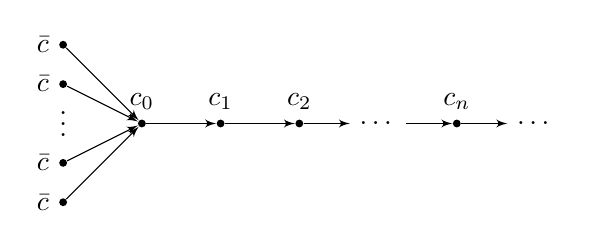
\begin{tikzpicture}
		\tikzset{vertex/.style = {shape=circle,fill,inner sep=1pt}}
		\tikzset{func/.style = {->,> = latex'}}

		% vertices \bar{c}
		\node[vertex,label=left:$\bar{c}$] (bc1) at (0,1){};
		\node[vertex,label=left:$\bar{c}$] (bc2) at (0,0.5){};
		\node at (0,0.1){$\vdots$};
		\node[vertex,label=left:$\bar{c}$] (bc3) at (0,-0.5){};
		\node[vertex,label=left:$\bar{c}$] (bc4) at (0,-1){};

		% vertices cn
		\node[vertex,label=above:$c_0$] (c0) at (1,0){};
		\node[vertex,label=above:$c_1$] (c1) at (2,0){};
		\node[vertex,label=above:$c_2$] (c2) at (3,0){};
		\node (c2dots) at (4,0){$\dots$};
		\node[vertex,label=above:$c_n$] (cn) at (5,0){};
		\node (cndots) at (6,0){$\dots$};

		%edges \bar{c} -> c_0
		\draw[func] (bc1) to (c0);
		\draw[func] (bc2) to (c0);
		\draw[func] (bc3) to (c0);
		\draw[func] (bc4) to (c0);
		% edge c0 -> c1 -> ...
		\draw[func] (c0) to (c1);
		\draw[func] (c1) to (c2);
		\draw[func] (c2) to (c2dots);
		\draw[func] (c2dots) to (cn);
		\draw[func] (cn) to (cndots);
	\end{tikzpicture}
	\caption{Graphical representation of the ``final" $f$}
	\label{ch4:fig:final-f-sketch}
\end{figure*}

The main idea is to pick a suitable $f$ in $F$ and define the sequence as the iterates $c_{n+1} = f(c_n)$. This function is sketched in figure \ref{ch4:fig:final-f-sketch}. The initial set of $\bar{c}$ mapped to $c_0$ is required to be able to apply lemma \ref{ch3:th:f-non-repr-pair} to all pairs $\{ \bar{c}, c_n \}$ and get that $c_{n+1} = f(c_n)$ is representable, since $f(\bar{c}) = c_0 \in R$.
The issue with this idea is that we don't have enough information on the sequence to pick such an $f$ at the beginning, so we actually bring along a (huge) list of candidate $f$ that all coincides on a prefix of the sequence. At step $n$, we pick a new element of the sequence among the possible images of $c_{n-1}$ through all candidate $f$ we have at that point, and discard all those that doesn't match the choice.

Actually, instead of directly consider functions, we represent them with elements $\bar{c}$ of $C$. Each element represent a function $f_{\bar{c}}$ that satisfies $f_{\bar{c}}(\bar{c}) = c_0$. Note that this function exists for ``enough" (that is, infinitely many) $\bar{c}$ because of the high surjectivity hypothesis. We call $E_n$ the set of $\bar{c}$ that represent functions that are ``valid" for the prefix up to $n$, ie. they map $c_{i}$ to $c_{i+1}$ for $0 \le i \le n - 1$. The core of the proof is an induction that proves that $E_n$ always contains infinitely many elements and that the newly chosen $c_n$ is different from all the others.

\begin{proof}
	Assume by contradiction that $A$ is non emptying for all $f \in F$. By hypothesis, $R$ isn't empty and thus we can take a $c_0 \in R$. We then construct recursively a sequence of representable elements $c_n$.

	Given an element $c \in C$, let
	\[
	NR(c) = C \setminus R(c) = \{ \bar{c} \in C \svert \{ c, \bar{c} \} \text{ is not representable} \}
	\]
	be the set of elements that are \textit{not} representable with it.

	Since $F$ is an highly surjective family, for an infinite amount of $\bar{c}$ there exists $f_{\bar{c}}$ such that $f_{\bar{c}}(\bar{c}) = c_0$.

	To ease presentation, we define here $E_n$, a set of element of $C$ that depends on the sequence $c_n$ we'll construct in the proof. Do note that the definition of $E_n$ only depends on elements of the sequence up to $c_n$.
	\begin{align*}
		E_n = \{\bar{c} \in C \svert & \forall\ 0 \le i \le n \ .\ \bar{c} \in NR(c_i), \\
		& f_{\bar{c}}(\bar{c}) = c_0, \\
		& \forall\ 0 \le i \le n - 1 \ .\ f_{\bar{c}}(c_i) = c_{i + 1} \}
	\end{align*}
	In the light of the introduction above, the first line is needed to apply lemma \ref{ch3:th:f-non-repr-pair} to the pair $\{ c_i, \bar{c} \}$ and get that $f_{\bar{c}}(c_i) = c_{i+1}$ is representable. The second one means that $\bar{c}$ actually represents $f_{\bar{c}}$, and the last is the requirement that $f_{\bar{c}}$ coincides on the prefix of the sequence up to $c_n$.

	We observe that the sequence $E_n$ can also be defined inductively by
	\begin{align*}
		E_0 &= \{ \bar{c} \in C \svert \bar{c} \in NR(c_0), f_{\bar{c}}(\bar{c}) = c_0 \} \\
		&= NR(c_0) \cap P(c_0)
	\end{align*}
	\begin{align*}
		E_{n+1} &= \{\ \bar{c} \in E_n \svert \bar{c} \in NR(c_{n+1}), f_{\bar{c}}(c_n) = c_{n+1} \} \\
		&= NR(c_{n+1}) \cap \{\ \bar{c} \in E_n \svert f_{\bar{c}}(c_n) = c_{n+1} \} \addtocounter{equation}{1}\tag{\theequation} \label{ch4:eq:En-relation}
	\end{align*}
	$E_0$ is the intersection of $NR(c_0)$ and the set of $\bar{c}$ for which there exists $f_{\bar{c}}$. Using lemma \ref{ch3:th:R-S-bound-integer-inf} to say $R(c_0)$ is finite and recalling that $P(c_0)$ is infinite (by high surjectivity), we observe that
	\begin{align*}
		E_0 = P(c_0) \cap NR(c_0) = P(c_0) \setminus (C \setminus NR(c_0)) = P(c_0) \setminus R(c_0)
	\end{align*}
	is infinite too.

	We then prove by induction on $n$ the following three statements: first $c_n$ is representable, ie. $c_n \in R$; second $E_n$ is infinite; third $c_n$ is different from all $c_i$ for $0 \le i \le n - 1$.
	We've already proved base case for $n = 0$: $c_0$ is representable by hypothesis, $E_0$ is infinite as shown above and the third condition is vacuous since there are no $0 \le i \le -1$.
	For the inductive step, assume the three hypothesis hold for $n$ and let us prove them for $n + 1$.
	Consider the set
	\[
	S = \{ f_{\bar{c}}(c_n) \svert \bar{c} \in E_n \}
	\]
	of candidate $c_{n+1}$.
	Since $c_n \in R$, $\bar{c} \in E_n \subseteq NR(c_n)$ and $f_{\bar{c}}(\bar{c}) = c_0 \in R$ (by inductive hypotheses) we can apply lemma \ref{ch3:th:f-non-repr-pair} to get $f_{\bar{c}}(c_n) \in R$ too, hence $S$ is a subset of $R$.
	Since $R$ is finite also $S$ must be, and by inductive hypothesis we know $E_n$ is infinite, so there must exists an element $c_{n+1}$ in $S$ such that an infinite amount of $\bar{c} \in E_n$ satisfies $f_{\bar{c}}(c_n) = c_{n+1}$. We observe that, as shown above, $c_{n+1} \in R$. Moreover we chose $c_{n+1}$ such that
	\[
	\{\ \bar{c} \in E_n \svert f_{\bar{c}}(c_n) = c_{n+1} \}
	\]
	is infinite, so we get
	\[
	\{\ \bar{c} \in E_n \svert f_{\bar{c}}(c_n) = c_{n+1} \} \cap NR(c_{n+1}) = \{\ \bar{c} \in E_n \svert f_{\bar{c}}(c_n) = c_{n+1} \} \setminus R(c_{n+1})
	\]
	is infinite too because $R(c_{n+1})$ is finite. But this, by equation \eqref{ch4:eq:En-relation} above, is exactly $E_{n+1}$.

	We only have to show that $c_{n+1} \neq c_i$ for all $0 \le i \le n$. Assume by contradiction that this is not the case: for some $0 \le j \le n$ it holds $c_{n+1} = c_j$, and let us distinguish two cases. If $j = 0$ we get $f_{\bar{c}}(c_n) = c_{n+1} = c_0 = f_{\bar{c}}(\bar{c})$, that would imply $c_n = \bar{c}$, but the former is representable and the latter is not, absurd. If otherwise $j > 0$ we get $f_{\bar{c}}(c_n) = c_{n+1} = c_j = f_{\bar{c}}(c_{j-1})$, that would imply $c_n = c_{j-1}$, that is not the case by inductive hypothesis. So $c_{n+1} \neq c_j$, and this concludes the inductive proof.

	By the induction above we have that all $c_n$, that are an infinite amount, are elements of $R$ and are all distinct. This yields the desired contradiction because $R$ is finite.
\end{proof}

Intuitively, if we were able to find the ``final" $f$ from the beginning, it would look like figure \ref{ch4:fig:final-f-sketch}: some $\bar{c}$, those for which that $f$ is $f_{\bar{c}}$, are mapped to $c_0$, and from there it just maps each $c_n$ to $c_{n+1}$. Do note that this is just an intuitive description: in fact, such an $f$ may not even exists (this correspond to the limit of $E_n$ being empty), but is indeed useful to visualize the proof.

A simple example of such a function family are constant sums over integers.
\begin{example}
	We take $C = \setZ$ and
	\[
	F = \{ \lambda x. x + n \svert n \in \setZ \}
	\]
	The family is highly surjective (actually $P(c) = \setZ$ for all $c$) and all these functions are injective, so it meets the hypothesis of the theorem.
\end{example}

Even though we've already proved that no abstract domain can be non emptying for all functions in this family $F$ in proposition \ref{ch3:th:ne-sum-nonexsistence-inf} in the previous chapter, it's important to note that this proof isn't a generalization of the proof of that proposition. In this proof, we iterate a single $f$ to build the entire sequence, while in that one we change the function every time, mapping the non representable $\bar{n}$ to the newly found representable $n_0 + t d$ to get that the image of $n_0$ through that function is representable too, as sketched in figure \ref{ch4:fig:ne-sum-inf-sketch}.

\begin{figure*}[ht]
	\centering
	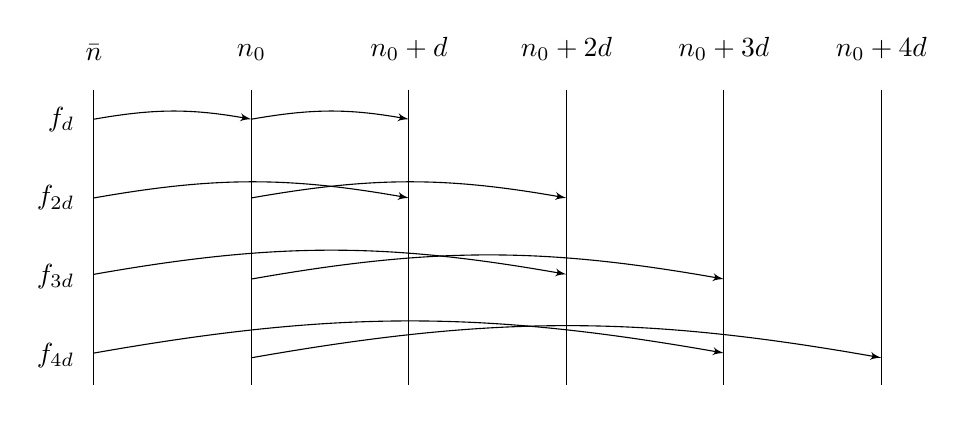
\begin{tikzpicture}
		\tikzset{vertex/.style = {shape=circle,fill,inner sep=1pt}}
		\tikzset{func/.style = {->,> = latex'}}

		% nodes cn
		\node[label=above:$\bar{n}$] (bnt) at (0, 2){};
		\node (bnb) at (0, -2){};
		\draw (bnt) to (bnb);

		\node[label=above:$n_0$] (n0t) at (2, 2){};
		\node (n0b) at (2, -2){};
		\draw (n0t) -- (n0b);

		\node[label=above:$n_0+d$] (n1t) at (4, 2){};
		\node (n1b) at (4, -2){};
		\draw (n1t) -- (n1b);

		\node[label=above:$n_0+2d$] (n2t) at (6, 2){};
		\node (n2b) at (6, -2){};
		\draw (n2t) -- (n2b);

		\node[label=above:$n_0+3d$] (n3t) at (8, 2){};
		\node (n3b) at (8, -2){};
		\draw (n3t) -- (n3b);

		\node[label=above:$n_0+4d$] (n4t) at (10, 2){};
		\node (n4b) at (10, -2){};
		\draw (n4t) -- (n4b);

		% f_0
		\node[label=left:$f_d$] at (0, 1.5){};
		\draw[func] (0, 1.5) to [bend left=10] (2, 1.5);
		\draw[func] (2, 1.5) to [bend left=10] (4, 1.5);

		% f_1
		\node[label=left:$f_{2d}$] at (0, 0.5){};
		\draw[func] (0, 0.5) to [bend left=10] (4, 0.5);
		\draw[func] (2, 0.5) to [bend left=10] (6, 0.5);

		% f_2
		\node[label=left:$f_{3d}$] at (0, -0.5){};
		\draw[func] (0, -0.47) to [bend left=10] (6, -0.47);
		\draw[func] (2, -0.53) to [bend left=10] (8, -0.53);

		% f_3
		\node[label=left:$f_{4d}$] at (0, -1.5){};
		\draw[func] (0, -1.47) to [bend left=10] (8, -1.47);
		\draw[func] (2, -1.53) to [bend left=10] (10, -1.53);
	\end{tikzpicture}
	\caption{Graphical representation of the proof of proposition \ref{ch3:th:ne-sum-nonexsistence-inf}}
	\label{ch4:fig:ne-sum-inf-sketch}
\end{figure*}

Another example are rational or real numbers, with sums or products, as shown for instance in this example
\begin{example}
	We take $C = \mathbb{Q} \setminus \{ 0 \}$ and
	\[
	F = \{ \lambda x. x \cdot q \svert q \in \mathbb{Q} \setminus \{ 0 \} \}
	\]
	The family is highly surjective since $P(c) = \mathbb{Q} \setminus \{ 0 \}$ for all $c$, and all these functions are invertible, hence injective.
\end{example}

An interesting observation about the proof is that we used injectivity of $f$ only to show that $c_{n+1} \neq c_i$, so any other condition that allows us to do so is a fine alternative. As an example, we present here the possibility that $f$ is acyclic instead of injective.
\begin{definition}[Acyclic function]
	Given a function $f$ from $C$ in itself we say that it's \textit{acyclic} if, for any finite sequence $c_0, c_1, \dots c_n$ of elements of $C$ of any length, it doesn't happen that
	\[
	f(c_0) = c_1, f(c_1) = c_2, \dots f(c_n) = c_0
	\]

	Is this holds for all sequences of length at least $2$, we say $f$ is \textit{almost acyclic}.
\end{definition}
If $f$ is acyclic the theorem holds: if for some $0 \le j \le n$ it were $c_{n+1} = c_j$, we would incur in the contradiction that $f$ has the cycle
\[
f(c_j) = c_{j+1}, \dots, f(c_n) = c_{n+1} = c_j
\]

However acyclicness is quite restrictive because it also considers sequences of length $1$, that means that $f$ can't have fixpoints. Almost acyclicness is useful exactly for this, but it's not enough on its own.
In particular, we can require almost acyclicness to functions in $F$ if we're also able to guarantee that $f(c_n) = c_{n+1} \neq c_n$, because for $0 \le j \le n - 1$ the same proof as above is still correct. A possible condition to enforce this is
\[
\forall c \in C.\ f(c) \neq c \implies f(f(c)) \neq f(c)
\]
This condition is enough since all $c_n$ are the image of something through $f$: for $n = 0$, $f(\bar{c})= c_0 \neq \bar{c}$, and for $n > 0$, $f(c_{n-1}) = c_n \neq c_{n-1}$.
This condition could be equivalently restated as any non-fixpoint of $f$ can't be mapped to a fixpoint, that is
\[
f(C \setminus \fix(f)) \subseteq C \setminus \fix(f)
\]
This condition is still restrictive, but is less so than acyclicness, that prevents fixpoints to exist at all.
Theorem \ref{ch4:th:non-empt-res-local-basic} could hence be generalized as
\begin{theorem}\label{ch4:th:non-empt-res-local}
	Let $F$ be an highly surjective function family from $C$ in itself such that all functions $f \in F$ satisfies at least one of the following conditions:
	\begin{itemize}
		\item $f$ is injective
		\item $f$ is acyclic
		\item $f$ is almost acyclic and $f(C \setminus \fix(f)) \subseteq C \setminus \fix(f)$
	\end{itemize}
	Assume also that $R$ isn't empty. Then $A$ can't be non emptying for all $f \in F$.
\end{theorem}

As an example of this more general version, we propose floating-point numbers and multiplications.
\begin{example}\label{ch4:ex:fp-numbers-local}
	We fix as concrete domain $C$ the set $\mathcal{F_+}$ of strictly positive floating-point numbers that can be represented with a fixed number of significant digits ($t$ bits) but with an arbitrary precision exponent. We make this choice in order to preserve characteristics of floating-point arithmetic but to have an infinite domain; a finite number of bits for exponents too would require a theorem for finite domains.\todo{Will I talk about this in a later section?} We limit ourselves to positive numbers since multiplications don't change signs, a discussion considering also negative numbers is completely analogous but takes twice as long to handle details of sign changes.

	Let $\cdot$ and $\odot$ denote respectively real product and its floating-point arithmetic approximation\todo{add ref}, and consider the function family
	\[
	F = \{ \lambda x . x \odot y \svert y \in \mathcal{F_+} \}
	\]

	First, we recall some basic properties about floating-point numbers and arithmetic. A floating-point number is defined by a significant $s$, of $t$ bits and satisfying $1 \le s < 2$, and an exponent $p$, and these correspond to the number $s \cdot 2^p$. If $\macheps$ is the machine epsilon and $\tilde{x}$ denotes the floating-point approximation of the real number $x$, then
	\[
	\left\lvert \frac{\tilde{x} - x}{x} \right\rvert < \macheps
	\]
	The smallest floating-point number greater than $1$ is $1 + 2^{-t+1}$. Analogously, the greatest floating-point number smaller than $1$ is $1 - 2^{-t}$. Moreover, $\macheps \le 2^{-t+1}$, hence the greatest number smaller than $1$ is at most $1 - \macheps / 2$.
	The floating-point multiplication is defined as\todo{fix the tilde because it's ugly}
	\[
	x \odot y = \widetilde{(x \cdot y)}
	\]
	and it is commutative and satisfies the following two properties.
	For any three floating point numbers $x$, $y$ and $z > 0$, if $x \le y$ also $x \odot z \le y \odot z$.
	For any two floating point numbers $x = s_1 \cdot 2^{p_1}$ and $y = s_2 \cdot 2^{p_2}$, the product $x \odot y = (s_1 \odot s_2) \cdot 2^{p_1 + p_2}$.

	We now show that $F$ meets the hypothesis of the theorem.
	The function family is highly surjective since, fixed $x = s \cdot 2^p$, we have that for all $n \ge 0$ the number
	$x \cdot 2^{-n} = s \cdot 2^{p-n}$ is in $\mathcal{F_+}$ and
	\[
	(x \cdot 2^{-n}) \odot (1 \cdot 2^{n}) = x
	\]
	hence $P(x) \supseteq \{ 1 \cdot 2^{-n} \svert n \ge 0 \}$ is infinite.
	For the second condition, if $y = 1 \cdot 2^{0}$ we have that the function $\lambda x. x \odot y$ is the identity, hence injective. So assume $y = s \cdot 2^p \neq 1 \cdot 2^0$ and let us show that $\lambda x. x \odot y$ is acyclic. Assume by contradiction it has a cycle $f(x_0) = x_1, f(x_1) = x_2, \dots, f(x_n) = x_0$. By monotonicity we have
	\[
	f(x) = x \odot y \ge x \odot 1 = x
	\]
	and then
	\[
	x_0 \le f(x_0) = x_1 \le f(x_1) = x_2 \le \dots \le x_n \le f(x_n) = x_0
	\]
	thus that all the elements of the cycle are equal, in particular $f(x_0) = x_0$. So we only have to show that such a function can't have a fixpoint.

	To do so, we distinguish four cases on $y = s \cdot 2^p$. In all four we assume $x_0 = s_0 \cdot 2^{p_0}$.
	If $p \ge 1$, since $s \ge 1$ we have
	\begin{align*}
		x_0 \odot y &= (s_0 \odot s) \cdot 2^{p_0 + p} \\
		&\ge (s_0 \odot 1) \cdot 2^{p_0 + 1} \\
		&= s_0 \cdot 2^{p_0} \cdot 2 > x_0
	\end{align*}
	If $p \le -2$, since $s < 2$ we have
	\begin{align*}
		x_0 \odot y &\le (s_0 \odot 2) \cdot 2^{p_0 + p} \\
		&\le (s_0 \odot 1) \cdot 2^{p_0 + p + 1} \\
		&= s_0 \cdot 2^{p_0} \cdot 2^{p + 1} \le x_0 / 2\\
	\end{align*}
	If $p = -1$ it must be the case that $s \cdot 2^{-1} \le 1 - \macheps / 2$, that is $s \le 2 - \macheps$, thus
	\[
	x_0 \odot y \le (s_0 \odot (2 - \macheps)) \cdot 2^{p_0 - 1}
	\]
	If $s_0 \odot (2 - \macheps) \ge s_0$ we would have
	\begin{align*}
		\macheps &> \left\lvert \frac{(s_0 \odot (2 - \macheps)) - s_0 \cdot (2 - \macheps)}{s_0 \cdot (2 - \macheps)} \right\rvert \\
		&\ge \left\lvert \frac{s_0 - s_0 \cdot (2 - \macheps)}{s_0 \cdot (2 - \macheps)} \right\rvert \\
		&= \left\lvert \frac{- 1 + \macheps}{2 - \macheps} \right\rvert \\
		&= \frac{1 - \macheps}{2 - \macheps} \ge \frac{1}{2} \ge \macheps\\
	\end{align*}
	where we assumed $\macheps \le 1/2$ for the last line, and this is a contradiction.
	Lastly, let us consider the case of $p = 0$. Since $y \neq 1$ it must be the case that $s \neq 1$ too, hence $s \ge 1 + 2^{-t+1}$. From this it follows
	\begin{align*}
		x_0 \odot y &= (s_0 \odot s) \cdot 2^{p_0 + p} \\
		&\ge (s_0 + s_0 \cdot 2^{-t+1}) \cdot 2^{p_0}
	\end{align*}
	Since $s \ge 1$ we have that $s_0 \cdot 2^{-t+1} \ge 2^{-t+1}$ and hence this is an increase in one of the bits of the machine representation of $s_0 \cdot s$, thus $s_0 \odot s \neq s$ because they differ in at least one bit.
	For example, assume $t = 4$, $s_0 = 1.011$ and $s = 1.001$ (that is its smallest possible value). Then the product is
	\begin{center}
		\begin{tabular}{c@{\;}c@{\,}c@{\,}c@{\,}c@{\,}c@{\,}c@{\,}c}
			& & & & 1. & 0 & 1 & 1 \\
			$\times$ & & & & 1. & 0 & 0 & 1 \\
			\hline
			& 0. & 0 & 0 & 1 & 0 & 1 & 1 \\
			$+$ & 1. & 0 & 1 & 1 & 0 & 0 & 0 \\
			\hline
			& 1. & 1 & 0 & 0 & 0 & 0 & 1
		\end{tabular}
	\end{center}
	so the result is represented (both with rounding and truncation) as $1.100$, that is different from $s_0 = 1.011$.

	In all four cases, the function has no fixpoint, and so it's acyclic. So this family meets hypothesis of theorem \ref{ch4:th:non-empt-res-local}: no abstract domain on floating-point numbers can be non emptying for all multiplications.
	Observe that theorem \ref{ch4:th:non-empt-res-local-basic} wasn't enough to prove this result, since in general these functions are not injective because of approximations. For instance both products
	\begin{center}
		\hfill
		\begin{tabular}{c@{\;}c@{\;}c@{\,}c@{\,}c@{\,}c@{\,}c@{\,}c@{\,}c}
			& & & & & 1. & 1 & 0 & 0 \\
			$\times$ & & & & & 1. & 1 & 0 & 0 \\
			\hline
			    & & 0. & 1 & 1 & 0 & 0 & 0 & 0\\
			$+$ & & 1. & 1 & 0 & 0 & 0 & 0 & 0 \\
			\hline
			  & 1 & 0. & 0 & 1 & 0 & 0 & 0 & 0
		\end{tabular}
		\hfill
		\begin{tabular}{c@{\;}c@{\;}c@{\,}c@{\,}c@{\,}c@{\,}c@{\,}c@{\,}c}
			& & & & & 1. & 1 & 0 & 1 \\
			$\times$ & & & & & 1. & 1 & 0 & 0 \\
			\hline
			    & & 0. & 1 & 1 & 0 & 1 & 0 & 0\\
			$+$ & & 1. & 1 & 0 & 1 & 0 & 0 & 0 \\
			\hline
			  & 1 & 0. & 0 & 1 & 1 & 1 & 0 & 0
		\end{tabular}
	\end{center}
	are approximated by the same floating-point number $1.001 \cdot 2^1$ but their first arguments differ by the last bit.
\end{example}

\section{Second result}
The second result we propose is instead more ``global", in the sense that it requires conditions on $F$ as a whole, and not on each $f$ on its own.

\begin{theorem}\label{ch4:th:non-empt-res-global}
	Let $F$ be a family of functions from $C$ in itself such that
	\begin{itemize}
		\item $F$ is highly surjective
		\item for all pair of elements $c, d \in C$ there exists at most a finite amount of $f \in F$ such that $f(d) = c$
		\item for all pair of an element $c \in C$ and a function $f \in F$, there exists at most a finite amount of elements $d \in C$ such that $f(d) = c$
	\end{itemize}
	Assume also that $R$ isn't empty. Then $A$ can't be non emptying for all $f \in F$.
\end{theorem}

The idea of the proof is that all these finiteness requirements makes it impossible to build enough $\bar{c}$ for which there exists $f_{\bar{c}}$ that maps them into $c_0$ (ie. $\bar{c} \in P(c_0)$), contradicting the hypothesis that $F$ is highly surjective. This may seem a little contradictory on its own (after all it is us that are requiring $F$ to satisfy all those conditions), but actually it is not because the proof also involves finiteness of $R$ and $R(c_0)$, that are enforced by the abstract domain. In fact we'll present an example of function family that meets those requirements.

The actual proof follows this idea in the opposite direction: starts from the (infinite) set $P(c_0)$ of $\bar{c}$ and propagates its infiniteness down to $R$.

\begin{proof}
	Assume by contradiction that $A$ is non emptying for all $f \in F$. By hypothesis, $R$ isn't empty and thus we can take a $c_0 \in R$.

	Since $F$ is an highly surjective family, $P(c_0)$ is infinite. Using lemma \ref{ch3:th:R-S-bound-integer-inf} to say that $R(c_0)$ is finite we can say that
	\begin{align*}
		E &= \{ \bar{c} \in C \svert \bar{c} \notin R(c_0), \exists f_{\bar{c}} \in F\ .\ f_{\bar{c}}(\bar{c}) = c_0 \} \\
		&= P(c_0) \setminus R(c_0)
	\end{align*}
	is infinite.

	Now fix a function $f \in F$, and let $J(f)$ be the set of $\bar{c}$ for which $f$ is exactly $f_{\bar{c}}$:
	\[
	J(f) = \{ \bar{c} \in C \setminus R(c_0) \svert f = f_{\bar{c}} \}
	\]

	Hence for all $\bar{c} \in J(f)$ we have $f(\bar{c}) = c_0$. By the third condition on $F$, this can be true for at most a finite amount of $\bar{c}$, that is $J(f)$ is finite.

	Now let $G$ be the set of functions in $F$ that are $f_{\bar{c}}$ for some $\bar{c} \in E$:
	\[
	G = \{ f \in F \svert \exists \bar{c} \in E\ .\ f = f_{\bar{c}} \}
	\]
	Clearly
	\[
	E = \bigcup\limits_{f \in G} J(f)
	\]
	But we know that $E$ is infinite while all $J(f)$ are finite, so $G$ must be infinite too.

	By lemma \ref{ch3:th:f-non-repr-pair}, for all $\bar{c} \in E$ we have $f_{\bar{c}}(c_0)$ is representable. This can be equivalently restated saying that for all $f \in G$, $f(c_0)$ is representable.
	So consider the set $I$ of all possible images of $c_0$ through functions in $G$:
	\[
	I = \{ f(c_0) \svert f \in G \}
	\]
	This set is a subset of $R$ because all its elements are representable.

	Clearly
	\[
	G = \bigcup\limits_{d \in I} \{ f \in G \svert f(c_0) = d \}
	\]
	But we know that $G$ is infinite and, for any $d \in C$, by the second condition on $F$ we have that
	\[
	\{ f \in F \svert f(c_0) = d \}
	\]
	is finite, and this is a superset of $\{ f \in G \svert f(c_0) = d \}$. So $I$ must be infinite too.

	However, this yields the desired contradiction: $I$ is infinite and is a subset of $R$, that is finite.
\end{proof}

As an example of such a family of functions we again propose floating-point numbers with multiplications:
\begin{example}
	Take $C = \mathcal{F} \setminus \{ 0 \}$ the set of non-zero floating-point numbers with $t$ bits significants, one bit sign and arbitrary precision exponents, and
	\[
	F = \{ \lambda x . x \odot y \svert y \in \mathcal{F} \setminus \{ 0 \} \}
	\]

	A straightforward adaptation of the argument of example \ref{ch4:ex:fp-numbers-local} (to take into account signs) shows that this family is highly surjective.
	Fixed two floating-point numbers $x, y$, we have that $y = f(x) = x \odot z$ only if
	\[
	\left\lvert \frac{y - (x \cdot z)}{x \cdot z} \right\rvert < \macheps
	\]
	that is
	\[
	\left\lvert\frac{y}{x}\right\rvert \frac{1}{1+\macheps} < \abs{z} < \left\lvert\frac{y}{x}\right\rvert \frac{1}{1-\macheps}
	\]
	This is a bounded interval since $x \neq 0$, and hence contains only a finite amount of floating-point numbers.
	Conversely, fixed a floating point $y$ and a function $f(x) = x \odot z$, we have that $y = x \odot z$ only if the same condition as above holds, that solved in $x$ becomes
	\[
	\left\lvert\frac{y}{z}\right\rvert \frac{1}{1+\macheps} < \abs{x} < \left\lvert\frac{y}{z}\right\rvert \frac{1}{1-\macheps}
	\]
	Again since $z \neq 0$ this is a bounded interval, thus proving the finiteness of the amount of floating-point $x$ that satisfies it.

	So, by means of theorem \ref{ch4:th:non-empt-res-global} above, we proved again that no abstract domain on floating-point numbers can be non emptying for all multiplications.
\end{example}

\section{Limitations}
\todo{reorganize}
The requirement that the function family $F$ is highly surjective is somewhat global: we require that \textit{all} possible $c$ has infinitely many preimages.
This is needed because first we fix the function family we want to analyse, then we can pick the abstract domain. Thinking of this as a game, player one fixes the function family and wants to show that there are no abstract domain able to analyse them, so player 2 thinks of a counterexample suited for that family. In fact, if there is even a single $c$ for which the condition doesn't hold, player 2 can actually construct such counterexample, as showed in the following proposition.
\todo{Move in another section "Limitations" with generalizations}
\begin{prop}
	For any fixed family $F$ of functions from $C$ in itself that is not highly onto, there exists an abstract domain $A_F$ such that:
	\begin{itemize}
		\item $A_F$ is finite
		\item all functions $f \in F$ are non emptying in $A_F$
	\end{itemize}
\end{prop}
\begin{proof}
	Since $F$ is not highly onto, there exists $c_0 \in C$ such that $P(c_0)$ is finite. We then define $A_F$ as follows.
	
	The only element of $C$ representable on its own is $c_0$ itself, ie. $R = \{ c_0 \}$.
	A pair of elements of $C$ is representable if and only if one of its elements is $c_0$ and the other is in $P(c_0)$. This also means that $R(c_0) = P(c_0)$.
	Subsets of $C$ with at least three elements are representable if and only if they are unions of representable pairs.
	
	Putting all together
	\[
	A_F = \{ \emptyset, \{ c_0 \} \} \cup \{ \{ c_0 \} \cup T \svert T \subseteq P(c_0) \}
	\]
	
	$A_F$ is a Moore family with respect to $\pow(C)^{\op}$ (it contains the maximal element, that is $\emptyset$, and is closed by union, that is meet in the opposite powerset), hence $A_F$ is a correct under-approximation abstract domain.
	
	Since $R(c_0) = P(c_0)$ is finite, we get that $A_F$ is finite too:
	\[
	\abs{A_F} = 2 + 2^{\abs{P(c_0)}}
	\]
	
	Now we want to show that any $f$ in $F$ is non emptying in $A_F$.
	We first observe that a subset $S \subseteq C$ is such that $\alpha(S) \neq \emptyset$ if and only if $c_0 \in S$. Suppose that $c_0 \in S$, then
	\[
	\alpha(S) \supseteq \alpha(\{ c_0 \}) = \{ c_0 \} \supset \emptyset
	\]
	Conversely, suppose that $\alpha(S) \neq \emptyset$. Since all elements of $A_F$ but the empty set contains $c_0$, by correctness we have
	\[
	c_0 \in \alpha(S) \subseteq S
	\]
	
	So fix now $S \subseteq C$ an element of the concrete domain. If $\alpha(S) = \emptyset$ then the non emptying condition is vacuously true, so assume $\alpha(S) \neq \emptyset$, or equivalently that $c_0 \in S$.
	Consider now $\alpha(f(S))$. If this is empty again the non emptying condition is vacuously true, so assume it is not. Again, this holds if and only if $c_0 \in f(S)$, that can be rewritten as $\exists d \in S\ .\ f(d) = c_0$. But by definition of $A_F$ we know this is equivalent to $d \in P(c_0) = R(c_0)$.
	Hence
	\begin{align*}
		&S \supseteq \{ c_0, d \} \\
		\implies& \alpha(S) \supseteq \alpha(\{ c_0, d \}) = \{ c_0, d \} \\
		\implies& f(\alpha(S)) \supseteq f(\{ c_0, d \}) \supseteq \{ f(d) \} = \{ c_0 \} \\
		\implies& f^{\flat}(\alpha(S)) = \alpha(f(\alpha(S))) \supseteq \alpha(\{ c_0 \}) = \{ c_0 \}
	\end{align*}
	Lines are motivated respectively by: monotonicity of $\alpha$ and representability of $\{ c_0, d \}$; monotonicity of $f$ and the fact that $f(d) = c_0$; monotonicity of $\alpha$ and representability of $\{ c_0 \}$. Also note that the implication chain above holds even if $d = c_0$.
	The last line implies $f^{\flat}(\alpha(S)) \neq \emptyset$, so $f$ is non emptying in $A_F$.
\end{proof}

We now show a simple example of the construction used in the proof
\begin{example}
	Fix the pair of functions $f(x) = x - 1$ and $g(x) = x - 2$ on $\setZ$, and let us build an under-approximating abstract domain for which these functions are non emptying. Following the proof of the previous proposition, we need an integer $n_0$ such that only a finite amount of integers can be mapped into it using either $f$ or $g$. Clearly any integer is fine, so let us fix $n_0 = 0$.
	
	The set $P(0)$ of integers that can be mapped into $0$ is simply $P(0) = \{ 1, 2 \}$. The abstract domain is then
	\[
	A_F = \{ \emptyset, \{ 0 \}, \{ 0, 1 \}, \{ 0, 2 \}, \{ 0, 1, 2 \} \}
	\]
	Both $f$ and $g$ are non emptying in $A_F$. A set $S$ isn't abstracted to $\emptyset$ if and only if it contains $0$, so fix one that does.
	For $f(S)$ not to be abstracted to $\emptyset$ we need also it to contain $0$, that means $1 \in S$. So
	\begin{align*}
		f^{\flat}(\alpha(S)) &= \alpha(f(\alpha(S))) \\
		&\supseteq \alpha(f(\alpha(\{ 0, 1 \}))) \\
		&= \alpha(f(\{ 0, 1 \})) \\
		&= \alpha(\{ -1, 0 \}) = \{ 0 \}
	\end{align*}
	The check for $g$ is analogous.
\end{example}

This proposition gives us one limit of approaches based on non emptying functions to show non existence of under-approximating abstract domains: whatever we do, we must fix enough functions to have high ontoness. This in particular means those approaches are ill suited to prove results where we focus on a single function.

In the following sections, we present two impossibility results. They share the same general structure: we fix a function family $F$ with some properties, assume that they are all non emptying in the abstract domain and that $R$ isn't empty. We need this last assumption in order to use lemma \ref{ch3:th:f-non-repr-pair}: if $R$ is empty we can't prove $f(\bar{c}) \in R$.

\todo{Scrivere bene le generalizzazioni e un po' di contesto}
Generalization of the above prop.
\begin{prop}
	Fix a family $F$ of functions from $\pow(C)$ in itself, and assume there is a set $S \subseteq C$ such that $P(S)$ is finite. Then there exists a finite abstract domain $A_F$ such that all functions $f \in F$ are non emptying in $A_F$.
\end{prop}
The proof is more or less the same.

``Dual" result of this (the other goes ``along" $F$, this goes ``backward").
\begin{prop}
	Fix a family $F$ of functions from $\pow(C)$ in itself, and for $S \subseteq C$ let $I(S)$ the set of all iterate images of $S$, that is the smallest subset of $\pow(C)$ such that
	\begin{align*}
		&S \in I(S) \\
		&f(T) \in I(S) \text{ for all } f \in F \text{, } T \in I(S)\\
	\end{align*}
	Assume there is a set $S \subseteq C$ such that $I(S)$ is finite. Then there exists a finite abstract domain $A_F$ such that all functions $f \in F$ are non emptying in $A_F$.
\end{prop}
The set $I(S)$ is just obtained from $S$ applying any possible sequence of functions in $F$ to it.


	\chapter{Conclusions and future works}

Some authors proposed \todo{ref} to use the union closure of well known over-approximation domains (eg. intervals) represented as sets of abstract elements in order to increase the precision of over-approximations. However this introduces overheads, hence the need for heuristics to decide when and how to reduce the size of this union. For instance, in the interval domain this means to decide when there are too many disjoint intervals, and then which ones should be merged into one, losing precision but gaining speed.
This approach also defines correct under-approximation domains, but again it needs heuristics to decide how to reduce the union size. In under-approximation, a safe possibility is to simply drop one interval from the union: the result is still an under-approximation of the real set of values. This idea correspond to application of the consequence rule of O'Hearn's incorrectness logic to drop a disjunction in the formula describing the final set of states, and is a perfect application of his sentence "For incorrectness reasoning, you must remember information as you go along a path, but you get to forget some of the paths."
The problem here is how to decide which intervals to drop, but a possibility would be to take inspiration from incorrectness logic and under-approximation tools not based on abstract interpretation. The question at that point would be whether there is any difference in using abstract interpretation or logic based tools, but it may be worth investigating.


	\printbibliography
	\addcontentsline{toc}{chapter}{Bibliography}
\end{document}
